%% LyX 2.3.1 created this file.  For more info, see http://www.lyx.org/.
%% Do not edit unless you really know what you are doing.
\documentclass[11pt,english,openright]{book}
\usepackage[T1]{fontenc}
\usepackage[latin9]{inputenc}
\usepackage[a4paper]{geometry}
\geometry{verbose,tmargin=3cm,bmargin=3.5cm,lmargin=4cm,rmargin=3cm}
\setcounter{secnumdepth}{3}
\setcounter{tocdepth}{3}
\usepackage{color}
\usepackage{babel}
\usepackage{float}
\usepackage{booktabs}
\usepackage{url}
\usepackage{amsmath}
\usepackage{amssymb}
\usepackage{graphicx}
\usepackage{setspace}
\onehalfspacing
\usepackage[unicode=true,pdfusetitle,
 bookmarks=true,bookmarksnumbered=false,bookmarksopen=false,
 breaklinks=false,pdfborder={0 0 1},backref=false,colorlinks=false]
 {hyperref}

\makeatletter

%%%%%%%%%%%%%%%%%%%%%%%%%%%%%% LyX specific LaTeX commands.
\providecommand{\LyX}{\texorpdfstring%
  {L\kern-.1667em\lower.25em\hbox{Y}\kern-.125emX\@}
  {LyX}}
\DeclareRobustCommand*{\lyxarrow}{%
\@ifstar
{\leavevmode\,$\triangleleft$\,\allowbreak}
{\leavevmode\,$\triangleright$\,\allowbreak}}
%% Because html converters don't know tabularnewline
\providecommand{\tabularnewline}{\\}
\floatstyle{ruled}
\newfloat{algorithm}{tbp}{loa}[chapter]
\providecommand{\algorithmname}{Algorithm}
\floatname{algorithm}{\protect\algorithmname}

%%%%%%%%%%%%%%%%%%%%%%%%%%%%%% User specified LaTeX commands.
% additional packages
\usepackage{tabularx}
\usepackage{setspace}
\usepackage{amsthm}
\usepackage{rotating}
\usepackage{caption}
\usepackage{epsfig}
\usepackage{indentfirst}
\usepackage{fancyhdr}
\usepackage{url}
\usepackage{cite}
\usepackage[normalem]{ulem}
\usepackage[table]{xcolor}
\usepackage{booktabs}
\usepackage{algpseudocode}

% this is a dirty fix for LTS version of Ubuntu/Kubuntu that has a
% very outdated "geometry" package
%%
%% This is file `geometry.sty',
%% generated with the docstrip utility.
%%
%% The original source files were:
%%
%% geometry.dtx  (with options: `package')
%% 
%% Copyright (C) 1996-2010
%% by Hideo Umeki <latexgeometry@gmail.com>
%% 
%% This work may be distributed and/or modified under the conditions of
%% the LaTeX Project Public License, either version 1.3c of this license
%% or (at your option) any later version. The latest version of this
%% license is in
%%    http://www.latex-project.org/lppl.txt
%% and version 1.3c or later is part of all distributions of LaTeX
%% version 2005/12/01 or later.
%% 
%% This work is "maintained" (as per the LPPL maintenance status)
%% by Hideo Umeki.
%% 
%% This work consists of the files geometry.dtx and
%% the derived files: geometry.{sty,ins,drv}, geometry-samples.tex.
%% 
\NeedsTeXFormat{LaTeX2e}
\ProvidesPackage{geometry}
  [2010/09/12 v5.6 Page Geometry]
\RequirePackage{keyval}%
\RequirePackage{ifpdf}%
\RequirePackage{ifvtex}%
\RequirePackage{ifxetex}%
\newif\ifGm@verbose
\newif\ifGm@landscape
\newif\ifGm@swap@papersize
\newif\ifGm@includehead
\newif\ifGm@includefoot
\newif\ifGm@includemp
\newif\ifGm@hbody
\newif\ifGm@vbody
\newif\ifGm@heightrounded
\newif\ifGm@showframe
\newif\ifGm@showcrop
\newif\ifGm@pass
\newif\ifGm@resetpaper
\newif\ifGm@layout
\newif\ifGm@newgm
\newcount\Gm@cnth
\newcount\Gm@cntv
\newcount\c@Gm@tempcnt
\newdimen\Gm@bindingoffset
\newdimen\Gm@wd@mp
\newdimen\Gm@odd@mp
\newdimen\Gm@even@mp
\newdimen\Gm@layoutwidth
\newdimen\Gm@layoutheight
\newdimen\Gm@layouthoffset
\newdimen\Gm@layoutvoffset
\newtoks\Gm@dimlist
\def\Gm@warning#1{\PackageWarningNoLine{geometry}{#1}}%
\def\ifGm@preamble#1{%
  \ifGm@newgm
   \Gm@warning{`#1': not available in `\string\newgeometry'; skipped}%
  \else
    \expandafter\@firstofone
  \fi}%
\def\Gm@Dhratio{1:1}% = left:right default for oneside
\def\Gm@Dhratiotwo{2:3}% = inner:outer default for twoside.
\def\Gm@Dvratio{2:3}% = top:bottom default
\def\Gm@Dhscale{0.7}%
\def\Gm@Dvscale{0.7}%
\def\Gm@dvips{dvips}%
\def\Gm@dvipdfm{dvipdfm}%
\def\Gm@pdftex{pdftex}%
\def\Gm@xetex{xetex}%
\def\Gm@vtex{vtex}%
\def\Gm@true{true}%
\def\Gm@false{false}%
\edef\Gm@orgpw{\the\paperwidth}%
\edef\Gm@orgph{\the\paperheight}%
\def\Gm@savelength#1{%
  \g@addto@macro\Gm@restore{\expandafter\noexpand\expandafter\csname
  #1\endcsname\expandafter=\expandafter\the\csname #1\endcsname\relax}}%
\def\Gm@saveboolean#1{%
  \csname if#1\endcsname
    \g@addto@macro\Gm@restore{\expandafter\noexpand\csname #1true\endcsname}%
  \else
    \g@addto@macro\Gm@restore{\expandafter\noexpand\csname #1false\endcsname}%
  \fi}%
\def\Gm@restore{}%
\def\Gm@save{%
  \Gm@savelength{paperwidth}%
  \Gm@savelength{paperheight}%
  \Gm@savelength{textwidth}%
  \Gm@savelength{textheight}%
  \Gm@savelength{evensidemargin}%
  \Gm@savelength{oddsidemargin}%
  \Gm@savelength{topmargin}%
  \Gm@savelength{headheight}%
  \Gm@savelength{headsep}%
  \Gm@savelength{topskip}%
  \Gm@savelength{footskip}%
  \Gm@savelength{baselineskip}%
  \Gm@savelength{marginparwidth}%
  \Gm@savelength{marginparsep}%
  \Gm@savelength{columnsep}%
  \Gm@savelength{hoffset}%
  \Gm@savelength{voffset}
  \Gm@savelength{Gm@layoutwidth}%
  \Gm@savelength{Gm@layoutheight}%
  \Gm@savelength{Gm@layouthoffset}%
  \Gm@savelength{Gm@layoutvoffset}%
  \Gm@saveboolean{@twocolumn}%
  \Gm@saveboolean{@twoside}%
  \Gm@saveboolean{@mparswitch}%
  \Gm@saveboolean{@reversemargin}}%
\def\Gm@initnewgm{%
  \Gm@passfalse
  \Gm@swap@papersizefalse
  \Gm@dimlist={}
  \Gm@hbodyfalse
  \Gm@vbodyfalse
  \Gm@heightroundedfalse
  \Gm@includeheadfalse
  \Gm@includefootfalse
  \Gm@includempfalse
  \let\Gm@width\@undefined
  \let\Gm@height\@undefined
  \let\Gm@textwidth\@undefined
  \let\Gm@textheight\@undefined
  \let\Gm@lines\@undefined
  \let\Gm@hscale\@undefined
  \let\Gm@vscale\@undefined
  \let\Gm@hmarginratio\@undefined
  \let\Gm@vmarginratio\@undefined
  \let\Gm@lmargin\@undefined
  \let\Gm@rmargin\@undefined
  \let\Gm@tmargin\@undefined
  \let\Gm@bmargin\@undefined
  \Gm@layoutfalse
  \Gm@layouthoffset\z@
  \Gm@layoutvoffset\z@
  \Gm@bindingoffset\z@}%
\def\Gm@initall{%
  \let\Gm@driver\@empty
  \let\Gm@truedimen\@empty
  \let\Gm@paper\@undefined
  \Gm@resetpaperfalse
  \Gm@landscapefalse
  \Gm@verbosefalse
  \Gm@showframefalse
  \Gm@showcropfalse
  \Gm@newgmfalse
  \Gm@initnewgm}%
\def\Gm@setdriver#1{%
  \expandafter\let\expandafter\Gm@driver\csname Gm@#1\endcsname}%
\def\Gm@unsetdriver#1{%
  \expandafter\ifx\csname Gm@#1\endcsname\Gm@driver\let\Gm@driver\@empty\fi}%
\def\Gm@setbool{\@dblarg\Gm@@setbool}%
\def\Gm@setboolrev{\@dblarg\Gm@@setboolrev}%
\def\Gm@@setbool[#1]#2#3{\Gm@doif{#1}{#3}{\csname Gm@#2\Gm@bool\endcsname}}%
\def\Gm@@setboolrev[#1]#2#3{\Gm@doifelse{#1}{#3}%
  {\csname Gm@#2\Gm@false\endcsname}{\csname Gm@#2\Gm@true\endcsname}}%
\def\Gm@doif#1#2#3{%
  \lowercase{\def\Gm@bool{#2}}%
  \ifx\Gm@bool\@empty
    \let\Gm@bool\Gm@true
  \fi
  \ifx\Gm@bool\Gm@true
  \else
    \ifx\Gm@bool\Gm@false
    \else
      \let\Gm@bool\relax
    \fi
  \fi
  \ifx\Gm@bool\relax
    \Gm@warning{`#1' should be set to `true' or `false'}%
  \else
    #3
  \fi}%
\def\Gm@doifelse#1#2#3#4{%
  \Gm@doif{#1}{#2}{\ifx\Gm@bool\Gm@true #3\else #4\fi}}%
\def\Gm@reverse#1{%
  \csname ifGm@#1\endcsname
  \csname Gm@#1false\endcsname\else\csname Gm@#1true\endcsname\fi}%
\def\Gm@defbylen#1#2{%
  \begingroup\setlength\@tempdima{#2}%
  \expandafter\xdef\csname Gm@#1\endcsname{\the\@tempdima}\endgroup}%
\def\Gm@defbycnt#1#2{%
  \begingroup\setcounter{Gm@tempcnt}{#2}%
  \expandafter\xdef\csname Gm@#1\endcsname{\the\value{Gm@tempcnt}}\endgroup}%
\def\Gm@sep@ratio#1:#2{\@tempcnta=#1\@tempcntb=#2}%
\def\Gm@setbyratio[#1]#2#3#4{% determine #4 by ratio
  \expandafter\Gm@sep@ratio\Gm@mratio\relax
  \if#1b
    \edef\@@tempa{\the\@tempcnta}%
    \@tempcnta=\@tempcntb
    \@tempcntb=\@@tempa\relax
  \fi
  \expandafter\setlength\expandafter\@tempdimb\expandafter
    {\csname Gm@#3\endcsname}%
  \ifnum\@tempcntb>\z@
    \multiply\@tempdimb\@tempcnta
    \divide\@tempdimb\@tempcntb
  \fi
  \expandafter\edef\csname Gm@#4\endcsname{\the\@tempdimb}}%
\def\Gm@detiv#1#2#3#4{% determine #4.
  \expandafter\setlength\expandafter\@tempdima\expandafter
    {\csname Gm@layout#1\endcsname}%
  \expandafter\setlength\expandafter\@tempdimb\expandafter
    {\csname Gm@#2\endcsname}%
  \addtolength\@tempdima{-\@tempdimb}%
  \expandafter\setlength\expandafter\@tempdimb\expandafter
    {\csname Gm@#3\endcsname}%
  \addtolength\@tempdima{-\@tempdimb}%
  \ifdim\@tempdima<\z@
    \Gm@warning{`#4' results in NEGATIVE (\the\@tempdima).%
    ^^J\@spaces `#2' or `#3' should be shortened in length}%
  \fi
  \expandafter\edef\csname Gm@#4\endcsname{\the\@tempdima}}%
\def\Gm@detiiandiii#1#2#3{% determine #2 and #3.
  \expandafter\setlength\expandafter\@tempdima\expandafter
    {\csname Gm@layout#1\endcsname}%
  \expandafter\setlength\expandafter\@tempdimb\expandafter
    {\csname Gm@#1\endcsname}%
  \addtolength\@tempdima{-\@tempdimb}%
  \ifdim\@tempdima<\z@
    \Gm@warning{`#2' and `#3' result in NEGATIVE (\the\@tempdima).%
                  ^^J\@spaces `#1' should be shortened in length}%
  \fi
  \ifx\Gm@mratio\@undefined
    \expandafter\Gm@sep@ratio\Gm@Dmratio\relax
  \else
    \expandafter\Gm@sep@ratio\Gm@mratio\relax
    \ifnum\@tempcntb>\z@\else
      \Gm@warning{margin ratio a:b should be non-zero; default used}%
      \expandafter\Gm@sep@ratio\Gm@Dmratio\relax
    \fi
  \fi
  \@tempdimb=\@tempdima
  \advance\@tempcntb\@tempcnta
  \divide\@tempdima\@tempcntb
  \multiply\@tempdima\@tempcnta
  \advance\@tempdimb-\@tempdima
  \expandafter\edef\csname Gm@#2\endcsname{\the\@tempdima}%
  \expandafter\edef\csname Gm@#3\endcsname{\the\@tempdimb}}%
\def\Gm@detall#1#2#3#4{%
  \@tempcnta\z@
  \if#1h
    \let\Gm@mratio\Gm@hmarginratio
    \edef\Gm@Dmratio{\if@twoside\Gm@Dhratiotwo\else\Gm@Dhratio\fi}%
  \else
    \let\Gm@mratio\Gm@vmarginratio
    \edef\Gm@Dmratio{\Gm@Dvratio}%
  \fi
  \if#1h
    \ifx\Gm@lmargin\@undefined\else\advance\@tempcnta4\relax\fi
    \ifGm@hbody\advance\@tempcnta2\relax\fi
    \ifx\Gm@rmargin\@undefined\else\advance\@tempcnta1\relax\fi
    \Gm@cnth\@tempcnta
  \else
    \ifx\Gm@tmargin\@undefined\else\advance\@tempcnta4\relax\fi
    \ifGm@vbody\advance\@tempcnta2\relax\fi
    \ifx\Gm@bmargin\@undefined\else\advance\@tempcnta1\relax\fi
    \Gm@cntv\@tempcnta
  \fi
  \ifcase\@tempcnta
    \if#1h
      \Gm@defbylen{width}{\Gm@Dhscale\Gm@layoutwidth}%
    \else
      \Gm@defbylen{height}{\Gm@Dvscale\Gm@layoutheight}%
    \fi
    \Gm@detiiandiii{#2}{#3}{#4}%
  \or
    \ifx\Gm@mratio\@undefined
      \if#1h
        \Gm@defbylen{width}{\Gm@Dhscale\Gm@layoutwidth}%
      \else
        \Gm@defbylen{height}{\Gm@Dvscale\Gm@layoutheight}%
      \fi
      \setlength\@tempdimc{\@nameuse{Gm@#4}}%
      \Gm@detiiandiii{#2}{#3}{#4}%
      \expandafter\let\csname Gm@#2\endcsname\@undefined
      \Gm@defbylen{#4}{\@tempdimc}%
    \else
      \Gm@setbyratio[f]{#1}{#4}{#3}%
    \fi
    \Gm@detiv{#2}{#3}{#4}{#2}%
  \or\Gm@detiiandiii{#2}{#3}{#4}%
  \or\Gm@detiv{#2}{#2}{#4}{#3}%
  \or
    \ifx\Gm@mratio\@undefined
      \if#1h
        \Gm@defbylen{width}{\Gm@Dhscale\Gm@layoutwidth}%
      \else
        \Gm@defbylen{height}{\Gm@Dvscale\Gm@layoutheight}%
      \fi
      \setlength\@tempdimc{\@nameuse{Gm@#3}}%
      \Gm@detiiandiii{#2}{#4}{#3}%
      \expandafter\let\csname Gm@#2\endcsname\@undefined
      \Gm@defbylen{#3}{\@tempdimc}%
    \else
      \Gm@setbyratio[b]{#1}{#3}{#4}%
    \fi
    \Gm@detiv{#2}{#3}{#4}{#2}%
  \or\Gm@detiv{#2}{#3}{#4}{#2}%
  \or\Gm@detiv{#2}{#2}{#3}{#4}%
  \or\Gm@warning{Over-specification in `#1'-direction.%
                  ^^J\@spaces `#2' (\@nameuse{Gm@#2}) is ignored}%
    \Gm@detiv{#2}{#3}{#4}{#2}%
  \else\fi}%
\def\Gm@clean{%
  \ifnum\Gm@cnth<4\let\Gm@lmargin\@undefined\fi
  \ifodd\Gm@cnth\else\let\Gm@rmargin\@undefined\fi
  \ifnum\Gm@cntv<4\let\Gm@tmargin\@undefined\fi
  \ifodd\Gm@cntv\else\let\Gm@bmargin\@undefined\fi
  \ifGm@hbody\else
    \let\Gm@hscale\@undefined
    \let\Gm@width\@undefined
    \let\Gm@textwidth\@undefined
  \fi
  \ifGm@vbody\else
    \let\Gm@vscale\@undefined
    \let\Gm@height\@undefined
    \let\Gm@textheight\@undefined
  \fi
  }%
\def\Gm@parse@divide#1#2#3#4{%
  \def\Gm@star{*}%
  \@tempcnta\z@
  \@for\Gm@tmp:=#1\do{%
    \expandafter\KV@@sp@def\expandafter\Gm@frag\expandafter{\Gm@tmp}%
    \edef\Gm@value{\Gm@frag}%
    \ifcase\@tempcnta\relax\edef\Gm@key{#2}%
      \or\edef\Gm@key{#3}%
      \else\edef\Gm@key{#4}%
    \fi
    \@nameuse{Gm@set\Gm@key false}%
    \ifx\empty\Gm@value\else
    \ifx\Gm@star\Gm@value\else
      \setkeys{Gm}{\Gm@key=\Gm@value}%
    \fi\fi
    \advance\@tempcnta\@ne}%
  \let\Gm@star\relax}%
\def\Gm@branch#1#2#3{%
  \@tempcnta\z@
  \@for\Gm@tmp:=#1\do{%
    \KV@@sp@def\Gm@frag{\Gm@tmp}%
    \edef\Gm@value{\Gm@frag}%
    \ifcase\@tempcnta\relax% cnta == 0
      \setkeys{Gm}{#2=\Gm@value}%
    \or% cnta == 1
      \setkeys{Gm}{#3=\Gm@value}%
    \else\fi
    \advance\@tempcnta\@ne}%
  \ifnum\@tempcnta=\@ne
    \setkeys{Gm}{#3=\Gm@value}%
  \fi}%
\def\Gm@magtooffset{%
  \@tempdima=\mag\Gm@truedimen sp%
  \@tempdimb=1\Gm@truedimen in%
  \divide\@tempdimb\@tempdima
  \multiply\@tempdimb\@m
  \addtolength{\hoffset}{1\Gm@truedimen in}%
  \addtolength{\voffset}{1\Gm@truedimen in}%
  \addtolength{\hoffset}{-\the\@tempdimb}%
  \addtolength{\voffset}{-\the\@tempdimb}}%
\def\Gm@setlength#1#2{%
  \let\Gm@len=\relax\let\Gm@td=\relax
  \edef\addtolist{\noexpand\Gm@dimlist=%
  {\the\Gm@dimlist \Gm@len{#1}{#2}}}\addtolist}%
\def\Gm@expandlengths{%
  \def\Gm@td{\Gm@truedimen}%
  \def\Gm@len##1##2{\setlength{##1}{##2}}%
  \the\Gm@dimlist}%
\def\Gm@setsize#1(#2,#3)#4{%
  \let\Gm@td\relax
  \expandafter\Gm@setlength\csname #1width\endcsname{#2\Gm@td #4}%
  \expandafter\Gm@setlength\csname #1height\endcsname{#3\Gm@td #4}%
  \ifGm@landscape\Gm@swap@papersizetrue\else\Gm@swap@papersizefalse\fi}%
\def\Gm@setpaper@ifpre#1{%
  \ifGm@preamble{#1}{\def\Gm@paper{#1}\@nameuse{Gm@#1}{paper}}}%
\@namedef{Gm@a0paper}#1{\Gm@setsize{#1}(841,1189){mm}}% ISO A0
\@namedef{Gm@a1paper}#1{\Gm@setsize{#1}(594,841){mm}}% ISO A1
\@namedef{Gm@a2paper}#1{\Gm@setsize{#1}(420,594){mm}}% ISO A2
\@namedef{Gm@a3paper}#1{\Gm@setsize{#1}(297,420){mm}}% ISO A3
\@namedef{Gm@a4paper}#1{\Gm@setsize{#1}(210,297){mm}}% ISO A4
\@namedef{Gm@a5paper}#1{\Gm@setsize{#1}(148,210){mm}}% ISO A5
\@namedef{Gm@a6paper}#1{\Gm@setsize{#1}(105,148){mm}}% ISO A6
\@namedef{Gm@b0paper}#1{\Gm@setsize{#1}(1000,1414){mm}}% ISO B0
\@namedef{Gm@b1paper}#1{\Gm@setsize{#1}(707,1000){mm}}% ISO B1
\@namedef{Gm@b2paper}#1{\Gm@setsize{#1}(500,707){mm}}% ISO B2
\@namedef{Gm@b3paper}#1{\Gm@setsize{#1}(353,500){mm}}% ISO B3
\@namedef{Gm@b4paper}#1{\Gm@setsize{#1}(250,353){mm}}% ISO B4
\@namedef{Gm@b5paper}#1{\Gm@setsize{#1}(176,250){mm}}% ISO B5
\@namedef{Gm@b6paper}#1{\Gm@setsize{#1}(125,176){mm}}% ISO B6
\@namedef{Gm@c0paper}#1{\Gm@setsize{#1}(917,1297){mm}}% ISO C0
\@namedef{Gm@c1paper}#1{\Gm@setsize{#1}(648,917){mm}}% ISO C1
\@namedef{Gm@c2paper}#1{\Gm@setsize{#1}(458,648){mm}}% ISO C2
\@namedef{Gm@c3paper}#1{\Gm@setsize{#1}(324,458){mm}}% ISO C3
\@namedef{Gm@c4paper}#1{\Gm@setsize{#1}(229,324){mm}}% ISO C4
\@namedef{Gm@c5paper}#1{\Gm@setsize{#1}(162,229){mm}}% ISO C5
\@namedef{Gm@c6paper}#1{\Gm@setsize{#1}(114,162){mm}}% ISO C6
\@namedef{Gm@b0j}#1{\Gm@setsize{#1}(1030,1456){mm}}% JIS B0
\@namedef{Gm@b1j}#1{\Gm@setsize{#1}(728,1030){mm}}% JIS B1
\@namedef{Gm@b2j}#1{\Gm@setsize{#1}(515,728){mm}}% JIS B2
\@namedef{Gm@b3j}#1{\Gm@setsize{#1}(364,515){mm}}% JIS B3
\@namedef{Gm@b4j}#1{\Gm@setsize{#1}(257,364){mm}}% JIS B4
\@namedef{Gm@b5j}#1{\Gm@setsize{#1}(182,257){mm}}% JIS B5
\@namedef{Gm@b6j}#1{\Gm@setsize{#1}(128,182){mm}}% JIS B6
\@namedef{Gm@ansiapaper}#1{\Gm@setsize{#1}(8.5,11){in}}%
\@namedef{Gm@ansibpaper}#1{\Gm@setsize{#1}(11,17){in}}%
\@namedef{Gm@ansicpaper}#1{\Gm@setsize{#1}(17,22){in}}%
\@namedef{Gm@ansidpaper}#1{\Gm@setsize{#1}(22,34){in}}%
\@namedef{Gm@ansiepaper}#1{\Gm@setsize{#1}(34,44){in}}%
\@namedef{Gm@letterpaper}#1{\Gm@setsize{#1}(8.5,11){in}}%
\@namedef{Gm@legalpaper}#1{\Gm@setsize{#1}(8.5,14){in}}%
\@namedef{Gm@executivepaper}#1{\Gm@setsize{#1}(7.25,10.5){in}}%
\@namedef{Gm@screen}#1{\Gm@setsize{#1}(225,180){mm}}%
\define@key{Gm}{paper}{\setkeys{Gm}{#1}}%
\let\KV@Gm@papername\KV@Gm@paper
\define@key{Gm}{a0paper}[true]{\Gm@setpaper@ifpre{a0paper}}%
\define@key{Gm}{a1paper}[true]{\Gm@setpaper@ifpre{a1paper}}%
\define@key{Gm}{a2paper}[true]{\Gm@setpaper@ifpre{a2paper}}%
\define@key{Gm}{a3paper}[true]{\Gm@setpaper@ifpre{a3paper}}%
\define@key{Gm}{a4paper}[true]{\Gm@setpaper@ifpre{a4paper}}%
\define@key{Gm}{a5paper}[true]{\Gm@setpaper@ifpre{a5paper}}%
\define@key{Gm}{a6paper}[true]{\Gm@setpaper@ifpre{a6paper}}%
\define@key{Gm}{b0paper}[true]{\Gm@setpaper@ifpre{b0paper}}%
\define@key{Gm}{b1paper}[true]{\Gm@setpaper@ifpre{b1paper}}%
\define@key{Gm}{b2paper}[true]{\Gm@setpaper@ifpre{b2paper}}%
\define@key{Gm}{b3paper}[true]{\Gm@setpaper@ifpre{b3paper}}%
\define@key{Gm}{b4paper}[true]{\Gm@setpaper@ifpre{b4paper}}%
\define@key{Gm}{b5paper}[true]{\Gm@setpaper@ifpre{b5paper}}%
\define@key{Gm}{b6paper}[true]{\Gm@setpaper@ifpre{b6paper}}%
\define@key{Gm}{c0paper}[true]{\Gm@setpaper@ifpre{c0paper}}%
\define@key{Gm}{c1paper}[true]{\Gm@setpaper@ifpre{c1paper}}%
\define@key{Gm}{c2paper}[true]{\Gm@setpaper@ifpre{c2paper}}%
\define@key{Gm}{c3paper}[true]{\Gm@setpaper@ifpre{c3paper}}%
\define@key{Gm}{c4paper}[true]{\Gm@setpaper@ifpre{c4paper}}%
\define@key{Gm}{c5paper}[true]{\Gm@setpaper@ifpre{c5paper}}%
\define@key{Gm}{c6paper}[true]{\Gm@setpaper@ifpre{c6paper}}%
\define@key{Gm}{b0j}[true]{\Gm@setpaper@ifpre{b0j}}%
\define@key{Gm}{b1j}[true]{\Gm@setpaper@ifpre{b1j}}%
\define@key{Gm}{b2j}[true]{\Gm@setpaper@ifpre{b2j}}%
\define@key{Gm}{b3j}[true]{\Gm@setpaper@ifpre{b3j}}%
\define@key{Gm}{b4j}[true]{\Gm@setpaper@ifpre{b4j}}%
\define@key{Gm}{b5j}[true]{\Gm@setpaper@ifpre{b5j}}%
\define@key{Gm}{b6j}[true]{\Gm@setpaper@ifpre{b6j}}%
\define@key{Gm}{ansiapaper}[true]{\Gm@setpaper@ifpre{ansiapaper}}%
\define@key{Gm}{ansibpaper}[true]{\Gm@setpaper@ifpre{ansibpaper}}%
\define@key{Gm}{ansicpaper}[true]{\Gm@setpaper@ifpre{ansicpaper}}%
\define@key{Gm}{ansidpaper}[true]{\Gm@setpaper@ifpre{ansidpaper}}%
\define@key{Gm}{ansiepaper}[true]{\Gm@setpaper@ifpre{ansiepaper}}%
\define@key{Gm}{letterpaper}[true]{\Gm@setpaper@ifpre{letterpaper}}%
\define@key{Gm}{legalpaper}[true]{\Gm@setpaper@ifpre{legalpaper}}%
\define@key{Gm}{executivepaper}[true]{\Gm@setpaper@ifpre{executivepaper}}%
\define@key{Gm}{screen}[true]{\Gm@setpaper@ifpre{screen}}%
\define@key{Gm}{paperwidth}{\ifGm@preamble{paperwidth}{%
  \def\Gm@paper{custom}\Gm@setlength\paperwidth{#1}}}%
\define@key{Gm}{paperheight}{\ifGm@preamble{paperheight}{%
  \def\Gm@paper{custom}\Gm@setlength\paperheight{#1}}}%
\define@key{Gm}{papersize}{\ifGm@preamble{papersize}{%
  \def\Gm@paper{custom}\Gm@branch{#1}{paperwidth}{paperheight}}}%
\define@key{Gm}{layout}{\Gm@layouttrue\@nameuse{Gm@#1}{Gm@layout}}%
\let\KV@Gm@layoutname\KV@Gm@layout
\define@key{Gm}{layoutwidth}{\Gm@layouttrue\Gm@setlength\Gm@layoutwidth{#1}}%
\define@key{Gm}{layoutheight}{\Gm@layouttrue\Gm@setlength\Gm@layoutheight{#1}}%
\define@key{Gm}{layoutsize}{\Gm@branch{#1}{layoutwidth}{layoutheight}}%
\define@key{Gm}{landscape}[true]{\ifGm@preamble{landscape}{%
  \Gm@doifelse{landscape}{#1}%
  {\ifGm@landscape\else\Gm@landscapetrue\Gm@reverse{swap@papersize}\fi}%
  {\ifGm@landscape\Gm@landscapefalse\Gm@reverse{swap@papersize}\fi}}}%
\define@key{Gm}{portrait}[true]{\ifGm@preamble{portrait}{%
  \Gm@doifelse{portrait}{#1}%
  {\ifGm@landscape\Gm@landscapefalse\Gm@reverse{swap@papersize}\fi}%
  {\ifGm@landscape\else\Gm@landscapetrue\Gm@reverse{swap@papersize}\fi}}}%
\define@key{Gm}{hscale}{\Gm@hbodytrue\edef\Gm@hscale{#1}}%
\define@key{Gm}{vscale}{\Gm@vbodytrue\edef\Gm@vscale{#1}}%
\define@key{Gm}{scale}{\Gm@branch{#1}{hscale}{vscale}}%
\define@key{Gm}{width}{\Gm@hbodytrue\Gm@defbylen{width}{#1}}%
\define@key{Gm}{height}{\Gm@vbodytrue\Gm@defbylen{height}{#1}}%
\define@key{Gm}{total}{\Gm@branch{#1}{width}{height}}%
\let\KV@Gm@totalwidth\KV@Gm@width
\let\KV@Gm@totalheight\KV@Gm@height
\define@key{Gm}{textwidth}{\Gm@hbodytrue\Gm@defbylen{textwidth}{#1}}%
\define@key{Gm}{textheight}{\Gm@vbodytrue\Gm@defbylen{textheight}{#1}}%
\define@key{Gm}{text}{\Gm@branch{#1}{textwidth}{textheight}}%
\let\KV@Gm@body\KV@Gm@text
\define@key{Gm}{lines}{\Gm@vbodytrue\Gm@defbycnt{lines}{#1}}%
\define@key{Gm}{includehead}[true]{\Gm@setbool{includehead}{#1}}%
\define@key{Gm}{includefoot}[true]{\Gm@setbool{includefoot}{#1}}%
\define@key{Gm}{includeheadfoot}[true]{\Gm@doifelse{includeheadfoot}{#1}%
  {\Gm@includeheadtrue\Gm@includefoottrue}%
  {\Gm@includeheadfalse\Gm@includefootfalse}}%
\define@key{Gm}{includemp}[true]{\Gm@setbool{includemp}{#1}}%
\define@key{Gm}{includeall}[true]{\Gm@doifelse{includeall}{#1}%
  {\Gm@includeheadtrue\Gm@includefoottrue\Gm@includemptrue}%
  {\Gm@includeheadfalse\Gm@includefootfalse\Gm@includempfalse}}%
\define@key{Gm}{ignorehead}[true]{%
  \Gm@setboolrev[ignorehead]{includehead}{#1}}%
\define@key{Gm}{ignorefoot}[true]{%
  \Gm@setboolrev[ignorefoot]{includefoot}{#1}}%
\define@key{Gm}{ignoreheadfoot}[true]{\Gm@doifelse{ignoreheadfoot}{#1}%
  {\Gm@includeheadfalse\Gm@includefootfalse}%
  {\Gm@includeheadtrue\Gm@includefoottrue}}%
\define@key{Gm}{ignoremp}[true]{%
  \Gm@setboolrev[ignoremp]{includemp}{#1}}%
\define@key{Gm}{ignoreall}[true]{\Gm@doifelse{ignoreall}{#1}%
  {\Gm@includeheadfalse\Gm@includefootfalse\Gm@includempfalse}%
  {\Gm@includeheadtrue\Gm@includefoottrue\Gm@includemptrue}}%
\define@key{Gm}{heightrounded}[true]{\Gm@setbool{heightrounded}{#1}}%
\define@key{Gm}{hdivide}{\Gm@parse@divide{#1}{lmargin}{width}{rmargin}}%
\define@key{Gm}{vdivide}{\Gm@parse@divide{#1}{tmargin}{height}{bmargin}}%
\define@key{Gm}{divide}{\Gm@parse@divide{#1}{lmargin}{width}{rmargin}%
  \Gm@parse@divide{#1}{tmargin}{height}{bmargin}}%
\define@key{Gm}{lmargin}{\Gm@defbylen{lmargin}{#1}}%
\define@key{Gm}{rmargin}{\Gm@defbylen{rmargin}{#1}}%
\let\KV@Gm@left\KV@Gm@lmargin
\let\KV@Gm@inner\KV@Gm@lmargin
\let\KV@Gm@innermargin\KV@Gm@lmargin
\let\KV@Gm@right\KV@Gm@rmargin
\let\KV@Gm@outer\KV@Gm@rmargin
\let\KV@Gm@outermargin\KV@Gm@rmargin
\define@key{Gm}{tmargin}{\Gm@defbylen{tmargin}{#1}}%
\define@key{Gm}{bmargin}{\Gm@defbylen{bmargin}{#1}}%
\let\KV@Gm@top\KV@Gm@tmargin
\let\KV@Gm@bottom\KV@Gm@bmargin
\define@key{Gm}{hmargin}{\Gm@branch{#1}{lmargin}{rmargin}}%
\define@key{Gm}{vmargin}{\Gm@branch{#1}{tmargin}{bmargin}}%
\define@key{Gm}{margin}{\Gm@branch{#1}{lmargin}{tmargin}%
  \Gm@branch{#1}{rmargin}{bmargin}}%
\define@key{Gm}{hmarginratio}{\edef\Gm@hmarginratio{#1}}%
\define@key{Gm}{vmarginratio}{\edef\Gm@vmarginratio{#1}}%
\define@key{Gm}{marginratio}{\Gm@branch{#1}{hmarginratio}{vmarginratio}}%
\let\KV@Gm@hratio\KV@Gm@hmarginratio
\let\KV@Gm@vratio\KV@Gm@vmarginratio
\let\KV@Gm@ratio\KV@Gm@marginratio
\define@key{Gm}{hcentering}[true]{\Gm@doifelse{hcentering}{#1}%
  {\def\Gm@hmarginratio{1:1}}{}}%
\define@key{Gm}{vcentering}[true]{\Gm@doifelse{vcentering}{#1}%
  {\def\Gm@vmarginratio{1:1}}{}}%
\define@key{Gm}{centering}[true]{\Gm@doifelse{centering}{#1}%
  {\def\Gm@hmarginratio{1:1}\def\Gm@vmarginratio{1:1}}{}}%
\define@key{Gm}{twoside}[true]{\Gm@doifelse{twoside}{#1}%
  {\@twosidetrue\@mparswitchtrue}{\@twosidefalse\@mparswitchfalse}}%
\define@key{Gm}{asymmetric}[true]{\Gm@doifelse{asymmetric}{#1}%
  {\@twosidetrue\@mparswitchfalse}{}}%
\define@key{Gm}{bindingoffset}{\Gm@setlength\Gm@bindingoffset{#1}}%
\define@key{Gm}{headheight}{\Gm@setlength\headheight{#1}}%
\define@key{Gm}{headsep}{\Gm@setlength\headsep{#1}}%
\define@key{Gm}{footskip}{\Gm@setlength\footskip{#1}}%
\let\KV@Gm@head\KV@Gm@headheight
\let\KV@Gm@foot\KV@Gm@footskip
\define@key{Gm}{nohead}[true]{\Gm@doifelse{nohead}{#1}%
  {\Gm@setlength\headheight\z@\Gm@setlength\headsep\z@}{}}%
\define@key{Gm}{nofoot}[true]{\Gm@doifelse{nofoot}{#1}%
  {\Gm@setlength\footskip\z@}{}}%
\define@key{Gm}{noheadfoot}[true]{\Gm@doifelse{noheadfoot}{#1}%
  {\Gm@setlength\headheight\z@\Gm@setlength\headsep
  \z@\Gm@setlength\footskip\z@}{}}%
\define@key{Gm}{footnotesep}{\Gm@setlength{\skip\footins}{#1}}%
\define@key{Gm}{marginparwidth}{\Gm@setlength\marginparwidth{#1}}%
\let\KV@Gm@marginpar\KV@Gm@marginparwidth
\define@key{Gm}{marginparsep}{\Gm@setlength\marginparsep{#1}}%
\define@key{Gm}{nomarginpar}[true]{\Gm@doifelse{nomarginpar}{#1}%
  {\Gm@setlength\marginparwidth\z@\Gm@setlength\marginparsep\z@}{}}%
\define@key{Gm}{columnsep}{\Gm@setlength\columnsep{#1}}%
\define@key{Gm}{hoffset}{\Gm@setlength\hoffset{#1}}%
\define@key{Gm}{voffset}{\Gm@setlength\voffset{#1}}%
\define@key{Gm}{offset}{\Gm@branch{#1}{hoffset}{voffset}}%
\define@key{Gm}{layouthoffset}{\Gm@setlength\Gm@layouthoffset{#1}}%
\define@key{Gm}{layoutvoffset}{\Gm@setlength\Gm@layoutvoffset{#1}}%
\define@key{Gm}{layoutoffset}{\Gm@branch{#1}{layouthoffset}{layoutvoffset}}%
\define@key{Gm}{twocolumn}[true]{%
  \Gm@doif{twocolumn}{#1}{\csname @twocolumn\Gm@bool\endcsname}}%
\define@key{Gm}{onecolumn}[true]{%
  \Gm@doifelse{onecolumn}{#1}{\@twocolumnfalse}{\@twocolumntrue}}%
\define@key{Gm}{reversemp}[true]{%
  \Gm@doif{reversemp}{#1}{\csname @reversemargin\Gm@bool\endcsname}}%
\define@key{Gm}{reversemarginpar}[true]{%
  \Gm@doif{reversemarginpar}{#1}{\csname @reversemargin\Gm@bool\endcsname}}%
\define@key{Gm}{driver}{\ifGm@preamble{driver}{%
  \edef\@@tempa{#1}\edef\@@auto{auto}\edef\@@none{none}%
  \ifx\@@tempa\@empty\let\Gm@driver\relax\else
  \ifx\@@tempa\@@none\let\Gm@driver\relax\else
  \ifx\@@tempa\@@auto\let\Gm@driver\@empty\else
  \setkeys{Gm}{#1}\fi\fi\fi\let\@@auto\relax\let\@@none\relax}}%
\define@key{Gm}{dvips}[true]{\ifGm@preamble{dvips}{%
  \Gm@doifelse{dvips}{#1}{\Gm@setdriver{dvips}}{\Gm@unsetdriver{dvips}}}}%
\define@key{Gm}{dvipdfm}[true]{\ifGm@preamble{dvipdfm}{%
  \Gm@doifelse{dvipdfm}{#1}{\Gm@setdriver{dvipdfm}}{\Gm@unsetdriver{dvipdfm}}}}%
\define@key{Gm}{pdftex}[true]{\ifGm@preamble{pdftex}{%
  \Gm@doifelse{pdftex}{#1}{\Gm@setdriver{pdftex}}{\Gm@unsetdriver{pdftex}}}}%
\define@key{Gm}{xetex}[true]{\ifGm@preamble{xetex}{%
  \Gm@doifelse{xetex}{#1}{\Gm@setdriver{xetex}}{\Gm@unsetdriver{xetex}}}}%
\define@key{Gm}{vtex}[true]{\ifGm@preamble{vtex}{%
  \Gm@doifelse{vtex}{#1}{\Gm@setdriver{vtex}}{\Gm@unsetdriver{vtex}}}}%
\define@key{Gm}{verbose}[true]{\ifGm@preamble{verbose}{\Gm@setbool{verbose}{#1}}}%
\define@key{Gm}{reset}[true]{\ifGm@preamble{reset}{%
  \Gm@doifelse{reset}{#1}{\Gm@restore@org\Gm@initall
  \ProcessOptionsKV[c]{Gm}\Gm@setdefaultpaper}{}}}%
\define@key{Gm}{resetpaper}[true]{\ifGm@preamble{resetpaper}{%
  \Gm@setbool{resetpaper}{#1}}}%
\define@key{Gm}{mag}{\ifGm@preamble{mag}{\mag=#1}}%
\define@key{Gm}{truedimen}[true]{\ifGm@preamble{truedimen}{%
  \Gm@doifelse{truedimen}{#1}{\let\Gm@truedimen\Gm@true}%
  {\let\Gm@truedimen\@empty}}}%
\define@key{Gm}{pass}[true]{\ifGm@preamble{pass}{\Gm@setbool{pass}{#1}}}%
\define@key{Gm}{showframe}[true]{\Gm@setbool{showframe}{#1}}%
\define@key{Gm}{showcrop}[true]{\Gm@setbool{showcrop}{#1}}%
\def\Gm@setdefaultpaper{%
  \ifx\Gm@paper\@undefined
    \Gm@setsize{paper}(\strip@pt\paperwidth,\strip@pt\paperheight){pt}%
    \Gm@setsize{Gm@layout}(\strip@pt\paperwidth,\strip@pt\paperheight){pt}%
    \Gm@swap@papersizefalse
  \fi}%
\def\Gm@adjustpaper{%
  \ifdim\paperwidth>\p@\else
    \PackageError{geometry}{%
    \string\paperwidth\space(\the\paperwidth) too short}{%
    Set a paper type (e.g., `a4paper').}%
  \fi
  \ifdim\paperheight>\p@\else
    \PackageError{geometry}{%
    \string\paperheight\space(\the\paperheight) too short}{%
    Set a paper type (e.g., `a4paper').}%
  \fi
  \ifGm@swap@papersize
    \setlength\@tempdima{\paperwidth}%
    \setlength\paperwidth{\paperheight}%
    \setlength\paperheight{\@tempdima}%
  \fi
  \ifGm@layout\else
    \setlength\Gm@layoutwidth{\paperwidth}%
    \setlength\Gm@layoutheight{\paperheight}%
  \fi}%
\def\Gm@checkmp{%
  \ifGm@includemp\else
    \@tempcnta\z@\@tempcntb\@ne
    \if@twocolumn
      \@tempcnta\@ne
    \else
      \if@reversemargin
        \@tempcnta\@ne\@tempcntb\z@
      \fi
    \fi
    \@tempdima\marginparwidth
    \advance\@tempdima\marginparsep
    \ifnum\@tempcnta=\@ne
      \@tempdimc\@tempdima
      \setlength\@tempdimb{\Gm@lmargin}%
      \advance\@tempdimc-\@tempdimb
      \ifdim\@tempdimc>\z@
        \Gm@warning{The marginal notes overrun the paper edge.^^J
        \@spaces Add \the\@tempdimc\space and more to the left margin}%
      \fi
    \fi
    \ifnum\@tempcntb=\@ne
      \@tempdimc\@tempdima
      \setlength\@tempdimb{\Gm@rmargin}%
      \advance\@tempdimc-\@tempdimb
      \ifdim\@tempdimc>\z@
        \Gm@warning{The marginal notes overrun the paper.^^J
        \@spaces Add \the\@tempdimc\space and more to the right margin}%
      \fi
    \fi
  \fi}%
\def\Gm@adjustmp{%
  \ifGm@includemp
    \@tempdimb\marginparwidth
    \advance\@tempdimb\marginparsep
    \Gm@wd@mp\@tempdimb
    \Gm@odd@mp\z@
    \Gm@even@mp\z@
    \if@twocolumn
      \Gm@wd@mp2\@tempdimb
      \Gm@odd@mp\@tempdimb
      \Gm@even@mp\@tempdimb
    \else
      \if@reversemargin
        \Gm@odd@mp\@tempdimb
        \if@mparswitch\else
          \Gm@even@mp\@tempdimb
        \fi
      \else
        \if@mparswitch
          \Gm@even@mp\@tempdimb
        \fi
      \fi
    \fi
  \fi}%
\def\Gm@adjustbody{
  \ifGm@hbody
    \ifx\Gm@width\@undefined
      \ifx\Gm@hscale\@undefined
        \Gm@defbylen{width}{\Gm@Dhscale\Gm@layoutwidth}%
      \else
        \Gm@defbylen{width}{\Gm@hscale\Gm@layoutwidth}%
      \fi
    \fi
    \ifx\Gm@textwidth\@undefined\else
      \setlength\@tempdima{\Gm@textwidth}%
      \ifGm@includemp
        \advance\@tempdima\Gm@wd@mp
      \fi
      \edef\Gm@width{\the\@tempdima}%
    \fi
  \fi
  \ifGm@vbody
    \ifx\Gm@height\@undefined
      \ifx\Gm@vscale\@undefined
        \Gm@defbylen{height}{\Gm@Dvscale\Gm@layoutheight}%
      \else
        \Gm@defbylen{height}{\Gm@vscale\Gm@layoutheight}%
      \fi
    \fi
    \ifx\Gm@lines\@undefined\else
      \ifdim\topskip<\ht\strutbox
        \setlength\@tempdima{\topskip}%
        \setlength\topskip{\ht\strutbox}%
        \Gm@warning{\noexpand\topskip was changed from \the\@tempdima\space
        to \the\topskip}%
      \fi
      \setlength\@tempdima{\baselineskip}%
      \multiply\@tempdima\Gm@lines
      \addtolength\@tempdima{\topskip}%
      \addtolength\@tempdima{-\baselineskip}%
      \edef\Gm@textheight{\the\@tempdima}%
    \fi
    \ifx\Gm@textheight\@undefined\else
      \setlength\@tempdima{\Gm@textheight}%
      \ifGm@includehead
        \addtolength\@tempdima{\headheight}%
        \addtolength\@tempdima{\headsep}%
      \fi
      \ifGm@includefoot
        \addtolength\@tempdima{\footskip}%
      \fi
      \edef\Gm@height{\the\@tempdima}%
    \fi
  \fi}%
\def\Gm@process{%
  \ifGm@pass
    \Gm@restore@org
  \else
    \Gm@@process
  \fi}%
\def\Gm@@process{%
  \Gm@expandlengths
  \Gm@adjustpaper
  \addtolength\Gm@layoutwidth{-\Gm@bindingoffset}%
  \Gm@adjustmp
  \Gm@adjustbody
  \Gm@detall{h}{width}{lmargin}{rmargin}%
  \Gm@detall{v}{height}{tmargin}{bmargin}%
  \setlength\textwidth{\Gm@width}%
  \setlength\textheight{\Gm@height}%
  \setlength\topmargin{\Gm@tmargin}%
  \setlength\oddsidemargin{\Gm@lmargin}%
  \addtolength\oddsidemargin{-1\Gm@truedimen in}%
  \ifGm@includemp
    \advance\textwidth-\Gm@wd@mp
    \advance\oddsidemargin\Gm@odd@mp
  \fi
  \if@mparswitch
    \setlength\evensidemargin{\Gm@rmargin}%
    \addtolength\evensidemargin{-1\Gm@truedimen in}%
    \ifGm@includemp
      \advance\evensidemargin\Gm@even@mp
    \fi
  \else
    \evensidemargin\oddsidemargin
  \fi
  \advance\oddsidemargin\Gm@bindingoffset
  \addtolength\topmargin{-1\Gm@truedimen in}%
  \ifGm@includehead
    \addtolength\textheight{-\headheight}%
    \addtolength\textheight{-\headsep}%
  \else
    \addtolength\topmargin{-\headheight}%
    \addtolength\topmargin{-\headsep}%
  \fi
  \ifGm@includefoot
    \addtolength\textheight{-\footskip}%
  \fi
  \ifGm@heightrounded
    \setlength\@tempdima{\textheight}%
    \addtolength\@tempdima{-\topskip}%
    \@tempcnta\@tempdima
    \@tempcntb\baselineskip
    \divide\@tempcnta\@tempcntb
    \setlength\@tempdimb{\baselineskip}%
    \multiply\@tempdimb\@tempcnta
    \advance\@tempdima-\@tempdimb
    \multiply\@tempdima\tw@
    \ifdim\@tempdima>\baselineskip
      \addtolength\@tempdimb{\baselineskip}%
    \fi
    \addtolength\@tempdimb{\topskip}%
    \textheight\@tempdimb
  \fi
  \advance\oddsidemargin\Gm@layouthoffset%
  \advance\evensidemargin\Gm@layouthoffset%
  \advance\topmargin\Gm@layoutvoffset%
  \addtolength\Gm@layoutwidth{\Gm@bindingoffset}%
  }% end of \Gm@@process
\def\Gm@detectdriver{%
  \ifx\Gm@driver\@empty
    \typeout{*geometry* driver: auto-detecting}%
    \ifpdf
      \Gm@setdriver{pdftex}%
    \else
      \Gm@setdriver{dvips}%
    \fi
    \ifvtex
      \Gm@setdriver{vtex}%
    \fi
    \ifxetex
      \Gm@setdriver{xetex}
    \fi
  \else
    \ifx\Gm@driver\Gm@xetex %%
      \ifxetex\else
        \Gm@warning{Wrong driver setting: `xetex'; trying `pdftex' driver}%
        \Gm@setdriver{pdftex}
      \fi
    \fi
    \ifx\Gm@driver\Gm@vtex
      \ifvtex\else
        \Gm@warning{Wrong driver setting: `vtex'; trying `dvips' driver}%
        \Gm@setdriver{dvips}%
      \fi
    \fi
  \fi
  \ifx\Gm@driver\relax
    \typeout{*geometry* detected driver: <none>}%
  \else
    \typeout{*geometry* detected driver: \Gm@driver}%
  \fi}%
\def\Gm@showparams#1{%
  \ifGm@verbose\expandafter\typeout\else\expandafter\wlog\fi
  {\Gm@logcontent{#1}}}%
\def\Gm@showdim#1{* \string#1=\the#1^^J}%
\def\Gm@showbool#1{\@nameuse{ifGm@#1}#1\space\fi}%
\def\Gm@logcontent#1{%
  *geometry* verbose mode - [ #1 ] result:^^J%
  \ifGm@pass * pass: disregarded the geometry package!^^J%
  \else
  * driver: \if\Gm@driver<none>\else\Gm@driver\fi^^J%
  * paper: \ifx\Gm@paper\@undefined<default>\else\Gm@paper\fi^^J%
  * layout: \ifGm@layout<custom>\else<same size as paper>\fi^^J%
  \ifGm@layout
  * layout(width,height): (\the\Gm@layoutwidth,\the\Gm@layoutheight)^^J%
  \fi
  * layoutoffset:(h,v)=(\the\Gm@layouthoffset,\the\Gm@layoutvoffset)^^J%
  \@ifundefined{Gm@lines}{}{* lines: \Gm@lines^^J}%
  \@ifundefined{Gm@hmarginratio}{}{* hratio: \Gm@hmarginratio^^J}%
  \@ifundefined{Gm@vmarginratio}{}{* vratio: \Gm@vmarginratio^^J}%
  \ifdim\Gm@bindingoffset=\z@\else
  * bindingoffset: \the\Gm@bindingoffset^^J\fi
  * modes: %
   \Gm@showbool{landscape}%
   \Gm@showbool{includehead}%
   \Gm@showbool{includefoot}%
   \Gm@showbool{includemp}%
   \if@twoside twoside\space\fi%
   \if@mparswitch\else\if@twoside asymmetric\space\fi\fi%
   \Gm@showbool{heightrounded}%
   \ifx\Gm@truedimen\@empty\else truedimen\space\fi%
   \Gm@showbool{showframe}%
   \Gm@showbool{showcrop}%
  ^^J%
  * h-part:(L,W,R)=(\Gm@lmargin, \Gm@width, \Gm@rmargin)^^J%
  * v-part:(T,H,B)=(\Gm@tmargin, \Gm@height, \Gm@bmargin)^^J%
  \fi
  \Gm@showdim{\paperwidth}%
  \Gm@showdim{\paperheight}%
  \Gm@showdim{\textwidth}%
  \Gm@showdim{\textheight}%
  \Gm@showdim{\oddsidemargin}%
  \Gm@showdim{\evensidemargin}%
  \Gm@showdim{\topmargin}%
  \Gm@showdim{\headheight}%
  \Gm@showdim{\headsep}%
  \Gm@showdim{\topskip}%
  \Gm@showdim{\footskip}%
  \Gm@showdim{\marginparwidth}%
  \Gm@showdim{\marginparsep}%
  \Gm@showdim{\columnsep}%
  * \string\skip\string\footins=\the\skip\footins^^J%
  \Gm@showdim{\hoffset}%
  \Gm@showdim{\voffset}%
  \Gm@showdim{\mag}%
  * \string\@twocolumn\if@twocolumn true\else false\fi^^J%
  * \string\@twoside\if@twoside true\else false\fi^^J%
  * \string\@mparswitch\if@mparswitch true\else false\fi^^J%
  * \string\@reversemargin\if@reversemargin true\else false\fi^^J%
  * (1in=72.27pt=25.4mm, 1cm=28.453pt)^^J}%
\def\Gm@cropmark(#1,#2,#3,#4){%
  \begin{picture}(0,0)
    \setlength\unitlength{1truemm}%
    \linethickness{0.25pt}%
    \put(#3,0){\line(#1,0){17}}%
    \put(0,#4){\line(0,#2){17}}%
  \end{picture}}%
\providecommand*\vb@xt@{\vbox to}%
\def\Gm@vrule{\vrule width 0.2pt height\textheight depth\z@}%
\def\Gm@hrule{\hrule height 0.2pt depth\z@ width\textwidth}%
\def\Gm@hruled{\hrule height\z@ depth0.2pt width\textwidth}%
\newcommand*{\Gm@vrules@mpi}{%
  \hb@xt@\@tempdima{\llap{\Gm@vrule}\ignorespaces
  \hskip \textwidth\Gm@vrule\hskip \marginparsep
  \llap{\Gm@vrule}\hfil\Gm@vrule}}%
\newcommand*{\Gm@vrules@mpii}{%
  \hb@xt@\@tempdima{\hskip-\marginparwidth\hskip-\marginparsep
  \llap{\Gm@vrule}\ignorespaces
  \hskip \marginparwidth\rlap{\Gm@vrule}\hskip \marginparsep
  \llap{\Gm@vrule}\hskip\textwidth\rlap{\Gm@vrule}\hss}}%
\newcommand*{\Gm@pageframes}{%
  \vb@xt@\z@{%
   \ifGm@showcrop
    \vb@xt@\z@{\vskip-1\Gm@truedimen in\vskip\Gm@layoutvoffset%
     \hb@xt@\z@{\hskip-1\Gm@truedimen in\hskip\Gm@layouthoffset%
      \vb@xt@\Gm@layoutheight{%
       \let\protect\relax
       \hb@xt@\Gm@layoutwidth{\Gm@cropmark(-1,1,-3,3)\hfil\Gm@cropmark(1,1,3,3)}%
       \vfil
       \hb@xt@\Gm@layoutwidth{\Gm@cropmark(-1,-1,-3,-3)\hfil\Gm@cropmark(1,-1,3,-3)}}%
     \hss}%
    \vss}%
   \fi%
   \ifGm@showframe
    \if@twoside
     \ifodd\count\z@
       \let\@themargin\oddsidemargin
     \else
       \let\@themargin\evensidemargin
     \fi
    \fi
    \moveright\@themargin%
    \vb@xt@\z@{%
     \vskip\topmargin\vb@xt@\z@{\vss\Gm@hrule}%
     \vskip\headheight\vb@xt@\z@{\vss\Gm@hruled}%
     \vskip\headsep\vb@xt@\z@{\vss\Gm@hrule}%
     \@tempdima\textwidth
     \advance\@tempdima by \marginparsep
     \advance\@tempdima by \marginparwidth
     \if@mparswitch
      \ifodd\count\z@
       \Gm@vrules@mpi
      \else
       \Gm@vrules@mpii
      \fi
     \else
      \Gm@vrules@mpi
     \fi
     \vb@xt@\z@{\vss\Gm@hrule}%
     \vskip\footskip\vb@xt@\z@{\vss\Gm@hruled}%
     \vss}%
    \fi%
  }}%
\def\ProcessOptionsKV{\@ifnextchar[%]
  {\@ProcessOptionsKV}{\@ProcessOptionsKV[]}}%
\def\@ProcessOptionsKV[#1]#2{%
  \let\@tempa\@empty
  \@tempcnta\z@
  \if#1p\@tempcnta\@ne\else\if#1c\@tempcnta\tw@\fi\fi
  \ifodd\@tempcnta
   \edef\@tempa{\@ptionlist{\@currname.\@currext}}%
  \else
    \@for\CurrentOption:=\@classoptionslist\do{%
      \@ifundefined{KV@#2@\CurrentOption}%
      {}{\edef\@tempa{\@tempa,\CurrentOption,}}}%
    \ifnum\@tempcnta=\z@
      \edef\@tempa{\@tempa,\@ptionlist{\@currname.\@currext}}%
    \fi
  \fi
  \edef\@tempa{\noexpand\setkeys{#2}{\@tempa}}%
  \@tempa
  \AtEndOfPackage{\let\@unprocessedoptions\relax}}%
\def\Gm@setkeys{\setkeys{Gm}}%
\def\Gm@processconfig{%
  \let\Gm@origExecuteOptions\ExecuteOptions
  \let\ExecuteOptions\Gm@setkeys
  \InputIfFileExists{geometry.cfg}{}{}
  \let\ExecuteOptions\Gm@origExecuteOptions}%
\Gm@save
\edef\Gm@restore@org{\Gm@restore}%
\Gm@initall
\Gm@processconfig
\ProcessOptionsKV[c]{Gm}%
\Gm@setdefaultpaper
\ProcessOptionsKV[p]{Gm}%
\Gm@process
\AtBeginDocument{%
  \Gm@savelength{paperwidth}%
  \Gm@savelength{paperheight}%
  \edef\Gm@restore@org{\Gm@restore}%
  \ifGm@resetpaper
    \edef\Gm@pw{\Gm@orgpw}%
    \edef\Gm@ph{\Gm@orgph}%
  \else
    \edef\Gm@pw{\the\paperwidth}%
    \edef\Gm@ph{\the\paperheight}%
  \fi
  \ifGm@pass\else
    \ifnum\mag=\@m\else
      \Gm@magtooffset
      \divide\paperwidth\@m
      \multiply\paperwidth\the\mag
      \divide\paperheight\@m
      \multiply\paperheight\the\mag
    \fi
  \fi
  \Gm@detectdriver
  \ifx\Gm@driver\Gm@xetex
    \@ifundefined{pdfpagewidth}{}{%
      \setlength\pdfpagewidth{\Gm@pw}%
      \setlength\pdfpageheight{\Gm@ph}}%
    \ifnum\mag=\@m\else
      \ifx\Gm@truedimen\Gm@true
        \setlength\paperwidth{\Gm@pw}%
        \setlength\paperheight{\Gm@ph}%
      \fi
    \fi
  \fi
  \ifx\Gm@driver\Gm@pdftex
    \@ifundefined{pdfpagewidth}{}{%
      \setlength\pdfpagewidth{\Gm@pw}%
      \setlength\pdfpageheight{\Gm@ph}}%
    \ifnum\mag=\@m\else
      \@tempdima=\mag sp%
      \@ifundefined{pdfhorigin}{}{%
        \divide\pdfhorigin\@tempdima
        \multiply\pdfhorigin\@m
        \divide\pdfvorigin\@tempdima
        \multiply\pdfvorigin\@m}%
      \ifx\Gm@truedimen\Gm@true
        \setlength\paperwidth{\Gm@pw}%
        \setlength\paperheight{\Gm@ph}%
      \fi
    \fi
  \fi
  \ifx\Gm@driver\Gm@vtex
    \@ifundefined{mediawidth}{}{%
      \mediawidth=\paperwidth
      \mediaheight=\paperheight}%
    \ifvtexdvi
      \AtBeginDvi{\special{papersize=\the\paperwidth,\the\paperheight}}%
    \fi
  \fi
  \ifx\Gm@driver\Gm@dvips
    \AtBeginDvi{\special{papersize=\the\paperwidth,\the\paperheight}}%
    \ifx\Gm@driver\Gm@dvips\ifGm@landscape
      \AtBeginDvi{\special{! /landplus90 true store}}%
    \fi\fi
  \else\ifx\Gm@driver\Gm@dvipdfm
    \ifcase\ifx\AtBeginShipoutFirst\relax\@ne\else
        \ifx\AtBeginShipoutFirst\@undefined\@ne\else\z@\fi\fi
      \AtBeginShipoutFirst{\special{papersize=\the\paperwidth,\the\paperheight}}%
    \or
      \AtBeginDvi{\special{papersize=\the\paperwidth,\the\paperheight}}%
    \fi
  \fi\fi
  \@tempswafalse
  \ifGm@showframe
    \@tempswatrue
  \else\ifGm@showcrop
    \@tempswatrue
  \fi\fi
  \if@tempswa
    \RequirePackage{atbegshi}%
      \AtBeginShipout{\setbox\AtBeginShipoutBox=\vbox{%
        \baselineskip\z@skip\lineskip\z@skip\lineskiplimit\z@
        \Gm@pageframes\box\AtBeginShipoutBox}}%
  \fi
  \Gm@save
  \edef\Gm@restore@pkg{\Gm@restore}%
  \ifGm@verbose\ifGm@pass\else\Gm@checkmp\fi\fi
  \Gm@showparams{preamble}%
  \let\Gm@pw\relax
  \let\Gm@ph\relax
  }% end of \AtBeginDocument
\newcommand{\geometry}[1]{%
  \Gm@clean
  \setkeys{Gm}{#1}%
  \Gm@process}%
\@onlypreamble\geometry
\DeclareRobustCommand\Gm@changelayout{%
  \setlength{\@colht}{\textheight}
  \setlength{\@colroom}{\textheight}%
  \setlength{\vsize}{\textheight}
  \setlength{\columnwidth}{\textwidth}%
  \if@twocolumn%
    \advance\columnwidth-\columnsep
    \divide\columnwidth\tw@%
    \@firstcolumntrue%
  \fi%
  \setlength{\hsize}{\columnwidth}%
  \setlength{\linewidth}{\hsize}}%
\newcommand{\newgeometry}[1]{%
  \clearpage
  \Gm@restore@org
  \Gm@initnewgm
  \Gm@newgmtrue
  \setkeys{Gm}{#1}%
  \Gm@newgmfalse
  \Gm@process
  \ifnum\mag=\@m\else\Gm@magtooffset\fi
  \Gm@changelayout
  \Gm@showparams{newgeometry}}%
\newcommand{\restoregeometry}{%
  \clearpage
  \Gm@restore@pkg
  \Gm@changelayout}%
\newcommand*{\savegeometry}[1]{%
  \Gm@save
  \expandafter\edef\csname Gm@restore@@#1\endcsname{\Gm@restore}}%
\newcommand*{\loadgeometry}[1]{%
  \clearpage
  \@ifundefined{Gm@restore@@#1}{%
    \PackageError{geometry}{%
    \string\loadgeometry : name `#1' undefined}{%
    The name `#1' should be predefined with \string\savegeometry}%
  }{\@nameuse{Gm@restore@@#1}%
  \Gm@changelayout}}%
\endinput
%%
%% End of file `geometry.sty'.


% fixes the page number of the first page of each chapter
\fancypagestyle{plain}{
\fancyhead{}
\renewcommand{\headrulewidth}{0pt}
\renewcommand{\footrulewidth}{0pt}
\fancyfoot[OC]{\begin{flushright}\thepage\end{flushright}}
}

% fancy headers for the thesis
\fancyhead{}
\fancyhead[LE]{\slshape \nouppercase \leftmark}
\fancyhead[RO]{\slshape \nouppercase \rightmark}
\fancyfoot[EC]{\begin{flushleft}\thepage\end{flushleft}}
\fancyfoot[OC]{\begin{flushright}\thepage\end{flushright}}
\renewcommand{\headrulewidth}{0.4pt}
\setlength{\headheight}{14pt}

\@ifundefined{showcaptionsetup}{}{%
 \PassOptionsToPackage{caption=false}{subfig}}
\usepackage{subfig}
\makeatother

\usepackage{listings}
\renewcommand{\lstlistingname}{Listing}

\begin{document}
\frontmatter
\pagestyle{empty}
\newgeometry{margin=3cm}\begin{titlepage}

\begin{center}
\Large{\textsc{Politecnico di Milano}}\\
\Large{Scuola di Ingegneria Industriale e dell'Informazione}\\
\large{Corso di Laurea Magistrale in Ingegneria Informatica}\\
\large{Dipartimento di Elettronica, Informazione e Bioingegneria}
\par\end{center}

\vspace{0.5cm}

\begin{center}
\begin{figure}[h]
\centering{}
\includegraphics[width=0.3\textwidth]{title-page/logo-polimi}
\end{figure}
\vspace{1cm}
\par\end{center}

\begin{center}
\LARGE{GEA\\
Gioco Educazione Alimentare}\vspace{2cm}
\par\end{center}

\begin{flushleft}
\begin{tabular}{ll}
Relatore:  & Prof. Franca GARZOTTO\tabularnewline
Correlatore:  & Ing. Mirko GELSOMINI\tabularnewline
\end{tabular}\vspace{1cm}
\par\end{flushleft}

\begin{flushright}
\begin{tabular}{ll}
Tesi di laurea di: & \tabularnewline
Federica BLANCO & Matr. 875487\tabularnewline
Giulia PENNATI & Matr. 882962\tabularnewline
\end{tabular}\vspace{4cm}
\par\end{flushright}

\begin{center}
{\large{}Anno Accademico 2017--2018}{\large\par}
\par\end{center}

\end{titlepage}
\restoregeometry

\cleardoublepage{}

\begin{flushright}
\emph{To someone very special\ldots
}\cleardoublepage{}
\par\end{flushright}

\chapter*{Acknowledgments}

\thispagestyle{empty}
\cleardoublepage{}

\chapter*{Abstract}

\thispagestyle{empty}Traduzione del sommario.
\cleardoublepage{}

\chapter*{Sommario}

\thispagestyle{empty}In italiano, descrizione NDD, scopo tesi, descrizione tecnologia usata(in breve), nome sistema sviluppato e collaborazione. (circa 1 pagina)\cleardoublepage\pagenumbering{roman}
\setcounter{page}{1}
\pagestyle{fancy}\tableofcontents{}\listoffigures
\listoftables
\listof{algorithm}{List of Algorithms}
\cleardoublepage\mainmatter
\renewcommand{\sectionmark}[1]{\markright{\thesection.\ #1}}
\renewcommand{\chaptermark}[1]{\markboth{\thechapter.\ #1}{}}

\chapter*{Introduction\label{chap:introduction}}

\addcontentsline{toc}{chapter}{Introduction}
\markboth{Introduction}{Introduction}\section{Food problems and their impact on childhood }
One of the main problems of modern society is the one related to nutrition. Nutrition has changed a lot in history thanks to the industrial development that allowed the massive production of foods that in the past were produced only by hand (and with high costs) and thanks also to scientific progresses that allowed the discovery of food conservation and their elaboration to obtain new kinds of food that are more suitable to our need. Montignac \cite{Lastoriadell'alimentazionedell'uomo.} also identifies other causes that brings the concept of "nutrition" to assume the current meaning, for example the habits evolution and the female emancipation that has changed the ancient vision of women as "landladies" and that has promoted the progression of the "ready meals" industry and therefore of pre-cocked and packaged meals that today are consumed increasingly. However, the main phenomenon that has taken place in our era is the one related to the globalization and standardization of destabilized north american eating habits that has promoted the global growth of fast-food, indicated by WHO (World Health Organization) as a "pandemic" since 1997 given its extraordinary expansion that carried also a lot of other problems.\\
Childhood obesity is surely one of the clearest examples of these diet's changes of the new millennium.
According to a seminar held by CB Ebbeling, DB Pawlak and DS Ludwig \cite{Childhoodobesity} childhood obesity is a phenomenon that has had a great increase in all the world in the last twenty years, as we can see from this diagram.\clearpage
\begin{figure}[H]
\centering
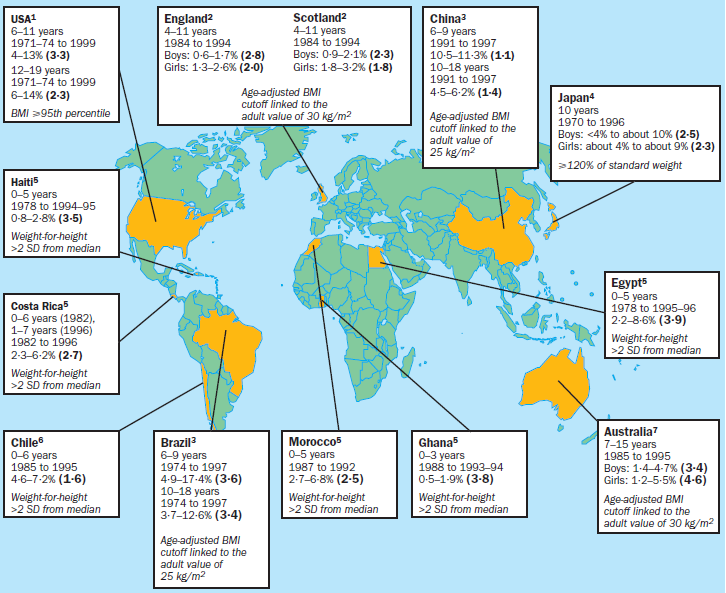
\includegraphics[width=13cm, height=10cm]{immagini/obesity.png}
\caption{Childhood obesity diagram}\label{fig:obesity}
\end{figure}
Historically, a fat child was seen as healthy because he was likely to survive better to illnesses and infections; however, excessive fatness has become one of the most diffused health problem in children. The three experts have underlined how the problem is most common in developed and industrialized nations in which diet has changed radically favouring foods containing saturated and trans fat and with high glycaemic index, typical of fast-food in which also bigger portions are served. Moreover, these foods are also poor of fibre, micronutrients and antioxidants that the body needs for a correct functioning of metabolism. The excessive consuming of these foods brings the child to have health problems such as heart diseases, vascular disorders, hypertension, chronic infiammations and diabete of type 2, illness that in the past was not present in teenagers, but that now has had a rapid spread.\linebreak 

Another important problem that affects the food safety of children is represented by allergies.
According to the data collected by AM Branum and SL Lukacs \cite{FoodallergyUSchildren} it is possible to observe an increasing in cases of all kinds of food allergies including milk, eggs, peanuts, tree nuts, fish, shellfish, soy and wheat of around the 18 per cent on individuals under the age of 18 from the 1997 onwards in US (but we have reasons to believe that this can also be found in all the industrialized world). Reactions to these foods may vary from small diseases to anaphylactic shock that, in severe cases, could lead to death.
The researches have also underlined how, in the same period analized previously, there was also an increasing of hospital discharges (clearly after an hospitalisation) due to allergic reactions as we can see from this barplot.
\begin{figure}[H]
\centering
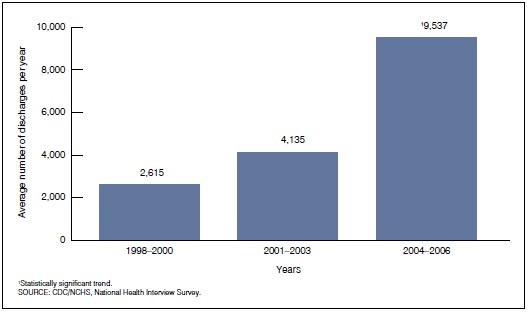
\includegraphics[width=10cm, height=7cm]{immagini/allergybarplot.png}
\caption{Allergy hospital discharges barplot}\label{fig:allergybarplot}
\end{figure}
All these problems that have been reinforced in recent years, lead us to think that it is necessary to support nutrition education and to make it a fundamental thing during childhood and adolescence, in order to empower everyone to a correct care of their health.

\section{Virtual Reality}
"Virtual Reality is electronic simulations of environments experienced via head mounted eye goggles and wired clothing enabling the end user to interact in realistic three-dimensional situations." (Coates, 1992)\\
We can define it using two variables: vividness, richness of an environments representation, and interactivity, extend to which a user can modify form and content of a mediated environment. The vividness is composed by sensory breadth, which refers to the number of sensory dimensions simultaneously presented,and sensory depth, which refers to the resolution within each of these perceptual channels; the interactivity instead is formed by speed, which refers to the rate at which input can be assimilated into the mediated environment, range, which refers to the number of possibilities for action at any given time and mapping, which refers to the ability of a system to map its controls to changes in the mediated environment in a natural and predictable manner.\cite{StefanSeipel} All of them, combined together, influence the telepresence that refers to a set of technologies which allow a user to feel as if he was present at a place different from his true location. So a "virtual reality" is defined as a real or simulated environment in which a perceiver experiences telepresence.\cite{JonathanSteuer}\\
\begin{figure}[H]
\centering
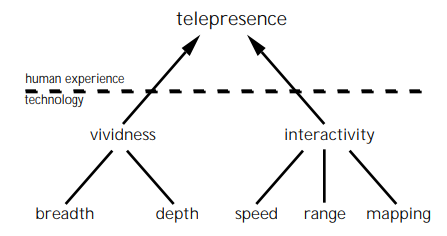
\includegraphics[width=8cm, height=5cm]{immagini/telepresence.png}
\caption{Telepresence infuencing variables}\label{fig:telepresence}
\end{figure}
We focus our project on Wearable Immersive Virtual Reality (WIVR). Immersive is the term that refers to the degree to which a virtual environment submerges the perceptual system of the user in computer-generated stimuli. The more the system captivates the sense and blocks out stimuli from the physical world the more the system is considered immersive.\cite{BioccaDelaney} Wearable indicates that the virtual environment is displayed in specialized small screen: we use a binocular head mounted displays (HMD) which allows to reach a fully immersive experience as we can see from this taxonomy by Muhanna \cite{Muhanna}.
\begin{figure}[H]
\centering
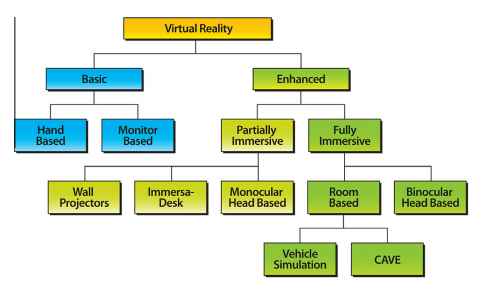
\includegraphics[width=10cm, height=7cm]{immagini/vrtaxonomy.png}
\caption{Virtual Reality taxonomy}\label{fig:vrtaxonomy}
\end{figure}
The HMD "trick" our brain using the principle of stereoscopic vision to simulate the perception of depth and to create 3D images and spaces, the VR has to generate two different images one for each eyes. The lenses of the visor augments the eyes in such a way we can converge the two scenes to obtain only one but that seems to be in the 3 dimensions space. Finally it can track the head movement so when we move it the space updates. 
\begin{figure}[H]
\centering
\begin{minipage}[c]{.40\textwidth}
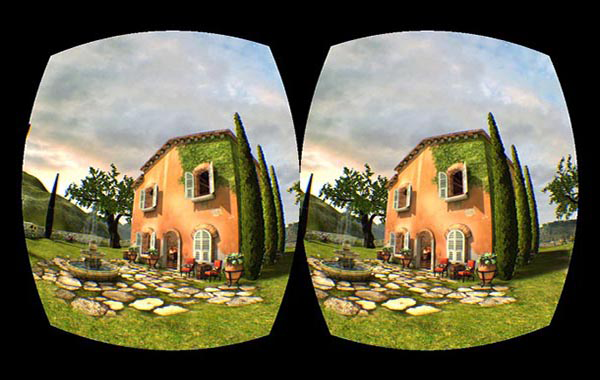
\includegraphics[width=1\textwidth]{immagini/immaginedoppia.png}
\end{minipage}%
\hspace{10mm}%
\begin{minipage}[c]{.40\textwidth}
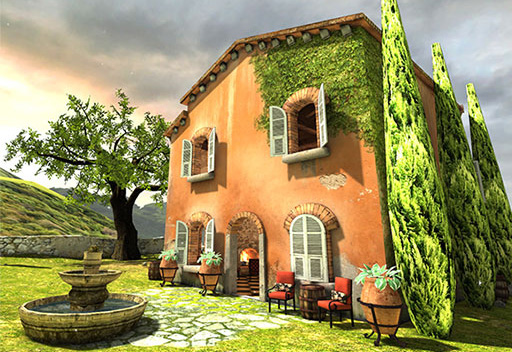
\includegraphics[width=1\textwidth]{immagini/immaginesingola.png}
\end{minipage}
\caption{Stereoscopic image and the correspondent 3D image}\label{fig:vrimages}
\end{figure}
Nowadays HMD are very popular and the costs are in a very big range from a cheap one, like Google Cardboard \cite{Cardboard}, to a more expensive one, like Samsung Gear VR \cite{Gear}, so the VR is for everyone. The VR is also used in a lot of different sectors as we can see in the following graph representing the investments in the 2015 taken from Digi-Capital \cite{DigiCapital}.
\begin{figure}[H]
\centering
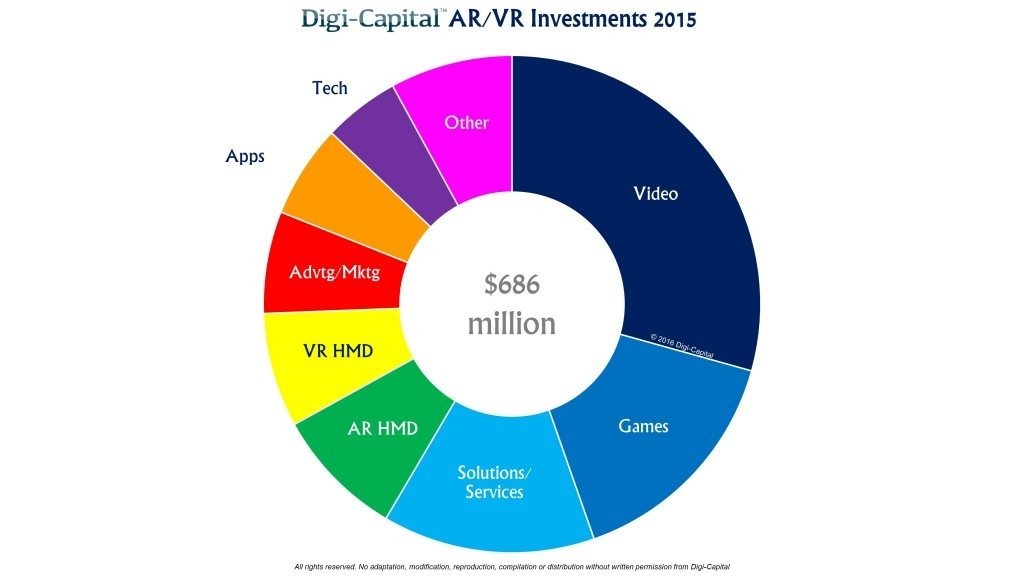
\includegraphics[width=15cm, height=7cm]{immagini/vrsectors.png}
\caption{Virtual Reality investments sectors}\label{fig:investments}
\end{figure}

\section{Touchscreen}
Touchscreen technology is something we have had for a longer time one can think. The first touchscreen device in fact was a radar built in capacitive way and dates back to around 1966. Its invention is due to E. A. Johnson and it works using a sheet of conductive, transparent material with a small current flowing on it. The central computer computes the current at each of the four corners, and when an objects touches the screen, a capacitor is formed between it and the platform and measuring again, the current on the corners the computer is able to approximately compute the point in which there was the touch.\\
At first this technology was abandoned, then in the first 2000s it was used on BlackBerry devices, but the major explosion of touchscreen devices is in the 2007, when Apple releases the first iPhone. \cite{Infante}
From that point on, touchscreen devices become increasingly used (as we can see from the graph below related to phones) and have had an explosive growth due to their main characteristic: the human computer interaction.
\begin{figure}[H]
\centering
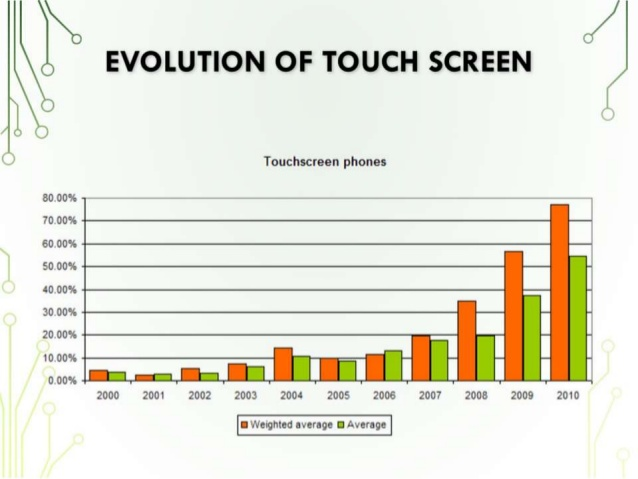
\includegraphics[width=12cm, height=9cm]{immagini/evolutouch.jpg}
\caption{Evolution of touchscreen}\label{fig:evolutouch}
\end{figure}
This interaction could be exploited by the fact that the user could touch directly what he wants without recurring to a third element (like a mouse) and this is particularly appealing because it makes the interaction more intuitive and allows a better usability of the system that is one of the main reasons of the success of this kind of devices. Moreover this improved usability will result in a easier training of people that learns faster and better with reduced costs due to the fact that this technology has grown a lot in recent years and it is no longer excessively expensive and resource-hungry \cite{Creed}.

\section{Neurodevelopmental Disorder}
The term neurodevelopmental disorder, NDD, contains within it all the conditions that are caused by a dysfunction of a part of the brain or nervous system that show some symptoms in the physical and psychological development of the child \cite{EPA}. Among the most common diseases we find Autism, ASD, attention deficit and hyperactivity, ADHD, and Down syndrome \cite{APA}. Children who suffer from these syndromes need help in developing cognitive abilities such as attention and language, social skills such as the ability to relate to others and personal and domestic autonomy skills. Dr. Dorothy Strickland, Department of Computer Science of North Carolina State University, in her treatise on the study of a VR application for autistic children \cite{Dorothy}, states that among the great benefits that can be found are: control on input stimuli, small changes to reach a generalization, safe learning situations, personalized treatment and learning with minimal human interference. In recent years there has been an increase in interest in the use of VR especially in the field of NDDs, \cite{Yufang} and \cite{Garzotto}, as, as stated in \cite{Strickland}, both the strength and limitations of Virtual Reality seem to adapt good for the needs that the learning tools for this type of disability require.\\
\\
As for the spread of these diseases take for example the autism on which there are no certain data, but there is agreement on the fact that the phenomenon is growing. According to the World Health Organization (WHO), ASD affects one child in 160 and recent estimates by the Cdc (Center for Disease Control) indicate that 3 million people are affected by this disorder in the US and about 60 million in world. According to estimates gathered by World Atlas, it would be Japan and Great Britain where autistic disorders occur more often.
\begin{figure}[H]
\centering
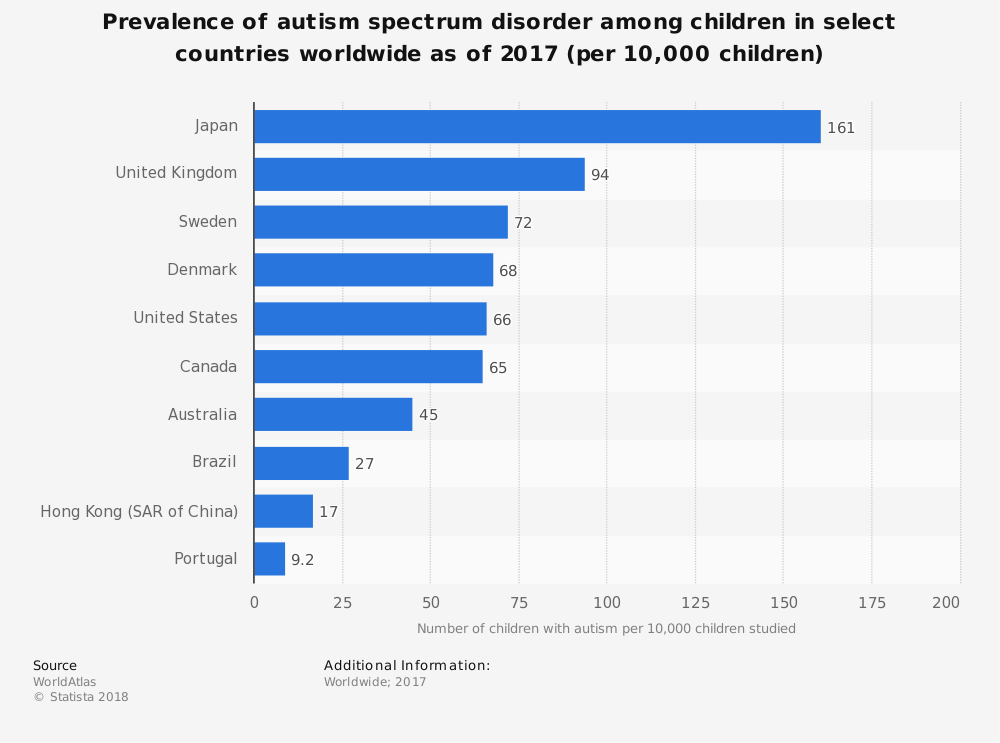
\includegraphics[width=15cm, height=10cm]{immagini/autismo.png}
\caption{Autism diffusion by World Atlas}\label{fig:autism}
\end{figure}

\section{Participatory Design and Therapy}
Over the past six decades, designer have been moving increasingly closer to the future users of what they design. In particular, design is becoming something that is more and more related to what the user needs, this imply the necessity of the collaboration between the experts in field (designers) and the final users (that are usually not experts) leading to what is now called co-design process.\\
The historic user-centred approach, in which designers thought as the user as final objective of their studies, but considered him as a passive entity, have been gradually substituted by the co-design process since the 1970s because people have been giving more importance to activities in which their opinion is required.
\begin{figure}[H]
\centering
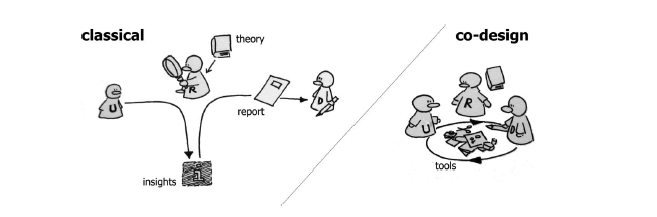
\includegraphics[width=16cm, height=5cm]{immagini/codesign.png}
\caption{Classical approach vs codesign approach}\label{fig:codesign}
\end{figure}
In the classical approach in fact, as we can see in the image above, there were different entities that collaborates to the final design of the product, but the user was considered a passive object of study: researches brings knowledge from theory and developed some more through the observation and interviews. Designer then apply this knowledge to conceptualize the final product. 
In co-creation approach, on the other hand, the roles get mixed-up: the user is involved as "expert of his/her experience" and plays a large role in the knowledge development idea generation and concept development \cite{Elizabeth}.\\
In the field of NDD, this could lead to multiple benefits: in particular, the target user perspective is taken into account since the early design phase and this allow to create something ad-hoc for this kind of people (for example the usage of simple words in explanations, the usage of certain kind of graphic stuffs and so on) and for the participants point of view, this could lead to a greater self-awareness and a more positive social behaviour.



\section{GEA and its Codesign process}
Considering the kind of target our application would have had and the importance of the subject we wanted to treat, we have decided to go through a co-design process which have involved both the final users and the therapists.\\
The starting point of our research were the kind of activities done in food education laboratory: in the first meeting we have observed how these activities are performed and then we have discussed with patients about these activities to hear their opinion and their engagement on them.\\
Then we have proposed our idea to create a virtual reality game based on the learning process provided by those activities that would have been used as a test to verify how much the patients have understood and assimilated the concepts.\\
These concepts have an important role in everyday life because they are related to self-awareness and autonomy in preparing and eating foods that some patients did not have initially and they have to improve their skills on them.\\
The patients have collaborated actively and with a lot of enthusiasm so we have decided to create a first abstract prototype of the application (with mockups and conceptual functioning).\\
In the second meeting we have first exposed our ideas about the three initial mini-games GEA was composed of to the therapist that evaluated their coherence with the food laboratory and their adequacy to the target end user it was thought for. \\
We understood the kind of difficulty required for the game also regarding the kind of interaction the game might have had, so we have changed small stuffs in our first idea, for example we have been informed that not all the users could read and that the presence of a lot of explanation was not useful for the game purpose, so we have thought how to improve the final usefulness of the game.\\
We have then implemented the first prototype of the game, that was tested from twb (ECCETERA, PER ORA IN SOSPESO)
\begin{figure}[H]
\centering
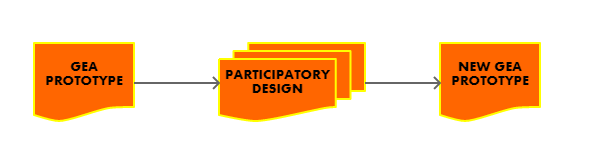
\includegraphics[width=12cm, height=4cm]{immagini/PD.png}
\caption{Phases of the work}\label{fig:phases}
\end{figure}

\section{GEA}
\subsection{Thesi Structure}
The thesis is organized as follows:
\begin{description}
\item[Chapter 1 (State of the art)] In this section we show all the technologies for Virtual Reality, explaining how they works and their relation with NDD people. We present also an instrument very useful for terapist that allow to replicate the smartphone's screen, Google Chromecast, and the touchscreen evolution. Finally we describe the projects already developed about food education.
\item[Chapter 2 (GEA: first prototype)] Here we describe how we elicitate the requirements, which are ours target groups, context, needs, constraints, goals. After that we show the UX design with description of all the app's pages and respective screenshot and flow diagram. Finally we briefly describe the implementation overview.
\item[Chapter 3 (First evaluation)]  
\item[Chapter 4 (GEA: second prototype)]
\item[Chapter 5 (Second evaluation)] 
\item[Chapter 6 (Value proposition)]
\item[Chapter 7 (Challenges)]  
\item[Chapter 8 (Implementation)] We present all the tools used to build up our application and the hardaware and software architecture description.
\item[Chapter 9 (Conclusion)]
\end{description}
At the end of the thesis, two appendices illustrate the materials used during the process
and shows some pictures of the process.
 
\subsection{Origin of the name and mascotte}
We decide to give the name GEA to our application because of two reasons. The first one is that Gea, in the greek mythology, was the personification of the Earth, the mother of all life so she is also the symbol of the nature that recalls the nutrition's topic. The second motivation is that in Italian Gea is the acronym of "Gioco Educazione Alimentare", which translated is "Food Education Game", in this way in the title there is the objective's explanation.\\
We have also designed a mascotte depicting a fairy of fruit and vegetables to leak the message that even the characters recognized by the community as positive eat healthy food; it is in fact dressed with elements such as strawberries like pigtails, pumpkin like a skirt, salad like top and cherries like little bows of shoes.
\begin{figure}[H]
\centering
\begin{minipage}[c]{.40\textwidth}

\includegraphics[width=1\textwidth]{immagini/geamasc.png}
\end{minipage}%
\hspace{10mm}%
\begin{minipage}[c]{.40\textwidth}

\includegraphics[width=1\textwidth]{immagini/GEA.png}
\end{minipage}
\caption{GEA logo and mascotte}\label{fig:logo}
\end{figure}

\chapter{First chapter\label{chap:first-chapter}}


\section{Lorem ipsum}

Lorem ipsum dolor sit amet, consectetur adipiscing elit. Quisque lectus
mi, aliquet ac lectus at, luctus ornare enim. Donec eleifend ornare
ante. Curabitur non adipiscing risus. Vivamus congue sem non magna
tristique, ut pellentesque diam ornare. Donec eget arcu congue, vulputate
nisl et, aliquam tellus. Morbi tincidunt odio quis mi hendrerit aliquet
sit amet sit amet lorem. Donec fringilla nec lectus nec lacinia. Aliquam
eu nunc euismod, tempus neque in, consequat velit. Duis arcu quam,
convallis quis ultricies vitae, semper in est. Aliquam congue sagittis
tortor, eget blandit lorem ullamcorper id. Maecenas venenatis nec
neque in consectetur. Nulla nisl turpis, elementum a enim interdum,
tincidunt vehicula tortor. Praesent pulvinar mi sit amet condimentum
placerat. Curabitur mollis libero non auctor condimentum. Suspendisse
ante lectus, sodales vel mauris vel, pharetra laoreet eros.

Nam lacinia nunc lorem, adipiscing ornare purus semper sit amet. Morbi
elementum augue vitae purus vehicula, ac varius leo sagittis. Vestibulum
eu orci in ipsum suscipit posuere. Nulla quis erat rhoncus risus rutrum
venenatis vel at lectus. Vivamus pharetra tempor rhoncus. Proin vitae
turpis vitae lacus ultrices lacinia eu ac nunc. Morbi id metus purus.
Pellentesque facilisis at arcu ut adipiscing. Etiam eu nisi hendrerit,
congue orci non, vehicula orci. Interdum et malesuada fames ac ante
ipsum primis in faucibus. Aenean porttitor eu velit sed pulvinar.
Class aptent taciti sociosqu ad litora torquent per conubia nostra,
per inceptos himenaeos. Maecenas ut pretium nisi, nec aliquam massa.
Maecenas vitae rhoncus lacus, non tempus turpis.

Nam luctus in nisi dignissim congue. Nullam dapibus dui sed ligula
euismod congue. Nulla vestibulum, justo a feugiat porttitor, massa
nunc molestie lectus, ultrices tempus turpis massa posuere augue.
Phasellus pulvinar vulputate ipsum, et eleifend sapien mollis vel.
Sed vitae eros id sapien dictum ultricies. Aliquam ultricies nisl
et bibendum imperdiet. Cras a sem eros. Quisque ut mauris a libero
hendrerit tincidunt ac ac mi. Mauris feugiat est sem, eu malesuada
ipsum faucibus id. Duis at ante et justo ullamcorper hendrerit sed
ut turpis. Donec eu dolor ac enim venenatis placerat venenatis vitae
velit. Curabitur lacus nisi, molestie id ligula vel, congue porta
felis. Nam eu aliquam justo. Mauris sapien nulla, accumsan id eros
a, porttitor interdum nunc.

Vestibulum aliquam et mauris imperdiet consectetur. Pellentesque convallis
metus dignissim neque tincidunt, egestas commodo odio rhoncus. Integer
purus leo, posuere non leo eget, aliquet condimentum neque. Quisque
non hendrerit quam. Phasellus sit amet neque quam. Suspendisse at
sollicitudin ante. Mauris fermentum turpis eget sem cursus tempor.
Fusce ac rutrum libero, sed adipiscing diam.

Praesent quis ultricies diam, in hendrerit nibh. Praesent diam dolor,
bibendum sit amet pharetra a, viverra vel tortor. Mauris id eleifend
diam. Maecenas tristique est massa, et lacinia ante tristique nec.
Praesent sapien odio, iaculis sollicitudin tristique vitae, mattis
non lacus. Ut vehicula enim pellentesque, mollis ante vitae, mollis
mauris. Aenean imperdiet tellus lorem, eget malesuada ante rhoncus
id. Pellentesque dignissim nisl id pretium condimentum. Sed congue
commodo massa in rhoncus. Phasellus elementum sollicitudin erat id
rhoncus. Fusce sem nunc, semper at tempor sit amet, congue nec orci.
Vivamus a egestas dui, vel viverra eros. Sed sit amet eros sit amet
nisi gravida ullamcorper. Nam rutrum in mi sit amet vulputate. Aenean
pellentesque velit eu nisi eleifend faucibus sit amet vel dui. Pellentesque
sapien est, auctor at fringilla vel, vehicula ut urna \cite{Dijkstra68Letters}.


\chapter{Second chapter\label{chap:second-chapter}}

These are general tips about few \LaTeX{} and \LyX{} functionalities.

\section{Copy and paste raw \protect\LaTeX{} code}

Sometimes it is necessary to insert raw \LaTeX{} code in your document,
\LyX{} has a dedicated environment for that (\textsf{Insert} \textsf{\lyxarrow}
\textsf{Tex code}). By using the paste command (\textsf{CTRL + V})
to copy text into that type of environment, you get as result that
everything is copied in a single line, all the carriage returns are
ignored. To paste exactly what you have copied, use the special paste
command which preserves the text formatting (\textsf{CTRL + SHIFT
+ V} or \textsf{Edit} \textsf{\lyxarrow{} Paste Special \lyxarrow Plain
Text}).

\section{Labels and cross-references\label{sec:label-and-cross}}

Labels are necessary to add cross-references in your thesis, use a
label for each element that you have to reference to (\textsf{Insert}
\textsf{\lyxarrow} \textsf{Label/Cross-reference}). These elements
are manly chapters, sections, subsections, figures, tables and algorithms.

This is Chapter \ref{chap:second-chapter}, Section \ref{sec:label-and-cross}.

\section{Figures}

Figures, but also tables and algorithms, must be placed inside a floating
environment. This type of \LaTeX{} environment is very useful and automagically
mix up text and images. Usually the \textsf{Here if possible} placement
option is good for all images (right click on \textsf{float: Figure}
then \textsf{Settings}). However, if the figure is not placed correctly
you may enable the \textsf{Ignore \LaTeX{} rules} option, usually that
option solves every problem.

Figure \ref{fig:image} shows an example of a very nice animal.

\begin{figure}[h]
\begin{centering}
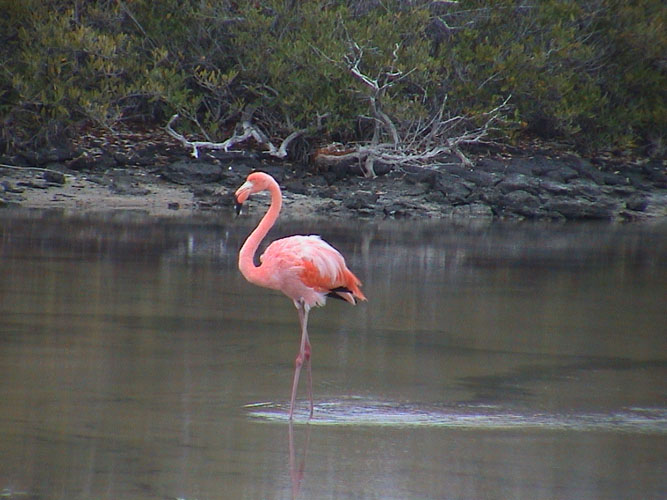
\includegraphics[width=0.5\columnwidth]{chapter-2/images/flamingo}
\par\end{centering}
\caption[Short caption of the figure]{\label{fig:image}Detailed caption of this marvelous animal}
\end{figure}
A rarely known feature of \LyX{} is the possibility to add the short
caption. The short caption is the description of the figure used in
the \textsf{List of Figures} section. Sometimes captions can be very
long, in this case it is better to use a shorter one that is more
readable in the page that lists all the figures. To add this caption,
right click on the description of figure, then \textsf{Insert short
title}.

It is not mandatory to add the short caption, it is only useful with
very long captions to ensure a better legibility of the \textsf{List
of Figures} section.

\subsection{Subfigures}

A very cool feature of \LaTeX 's figures is the possibility to have
subfigures. For example, if there are two figures that represent the
result of a test executed with two different values of a parameter,
then a subfigure is a good way to organize the images.

Figure \ref{fig:subfig-fauna} is an example of these subfigures.
References can be added to either the whole figure (Figure \ref{fig:subfig-fauna})
or each subfigure (Figure \ref{fig:fauna-squirrel} and Figure \ref{fig:fauna-peacock}).

\begin{figure}[h]
\hfill{}\subfloat[\label{fig:fauna-squirrel}A nice squirrel]{\centering{}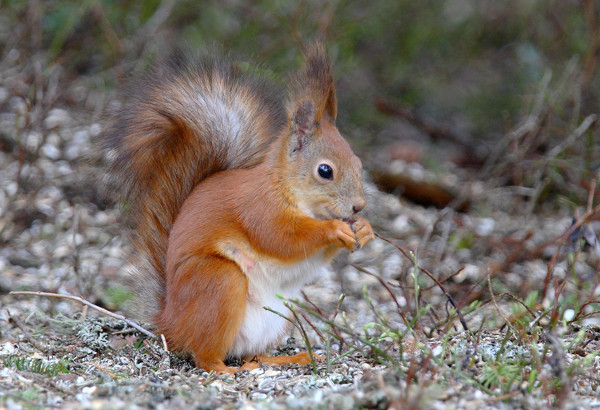
\includegraphics[width=0.45\columnwidth]{chapter-2/images/squirrel}}\hfill{}\subfloat[\label{fig:fauna-peacock}A beautiful peacock]{\centering{}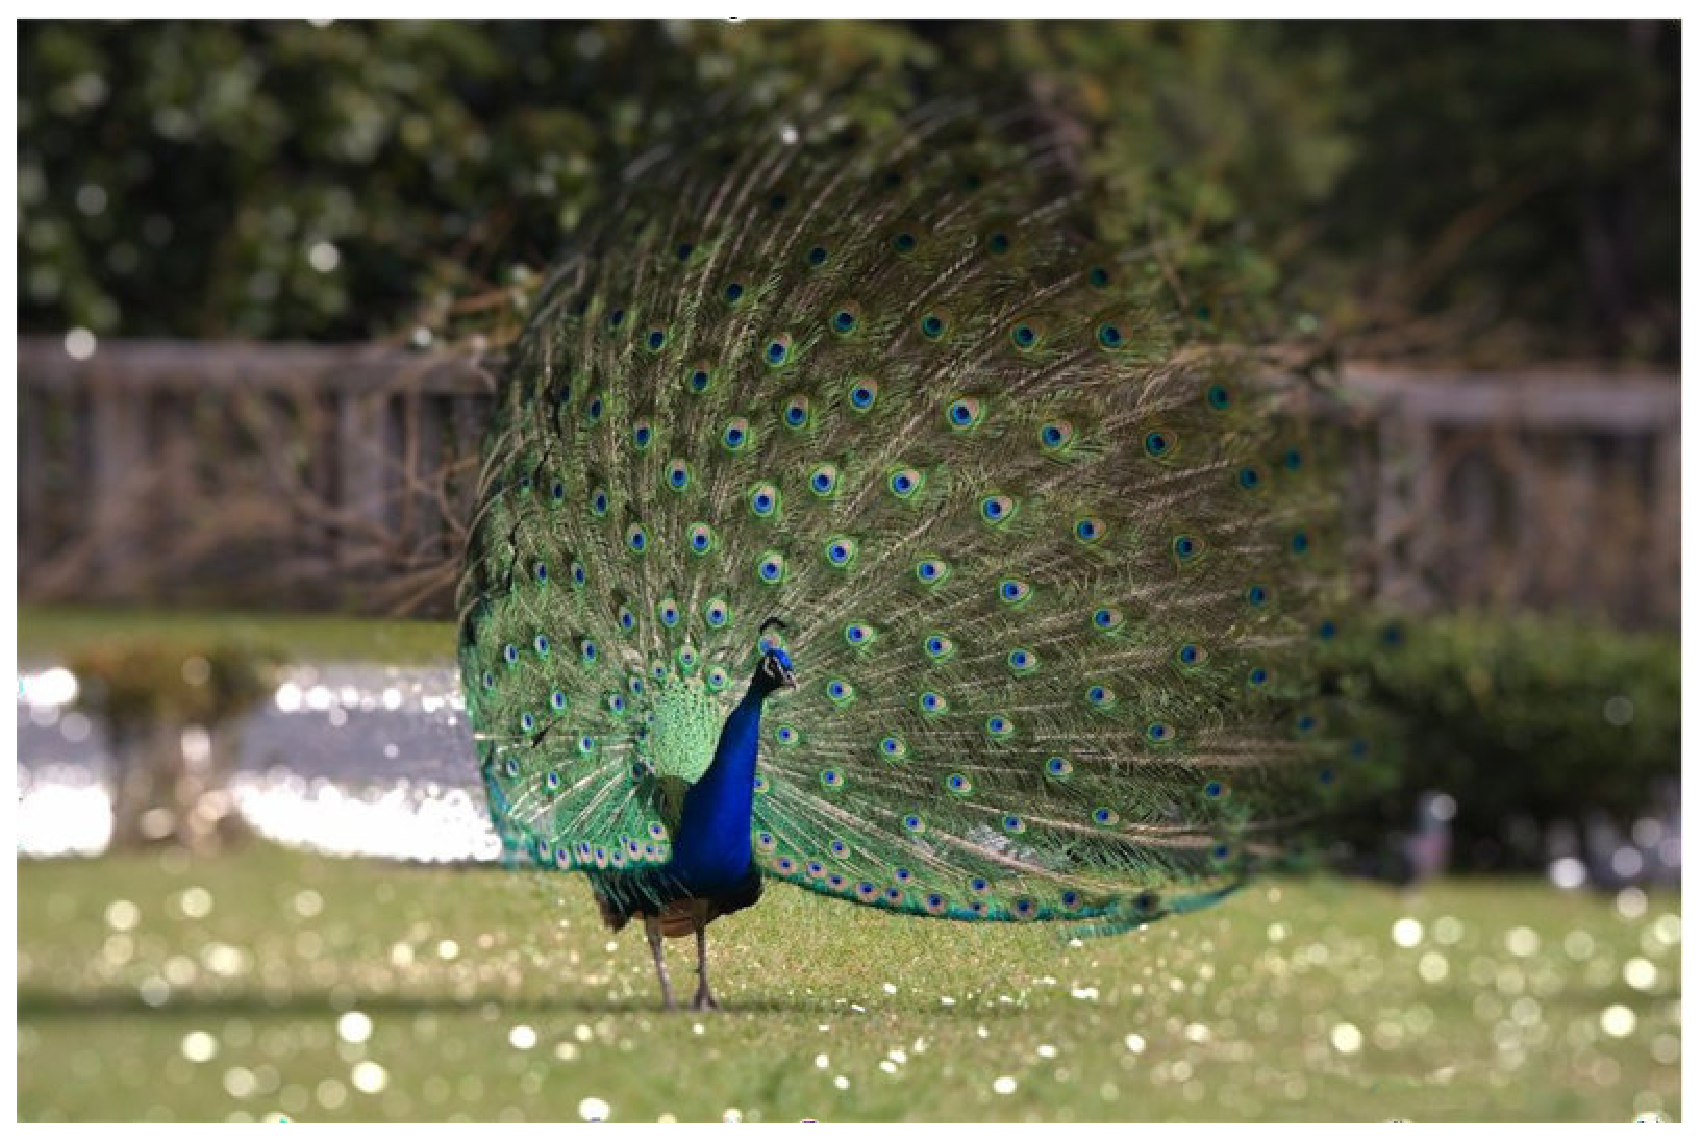
\includegraphics[width=0.45\columnwidth]{chapter-2/images/peacock}}\hfill{}

\caption{\label{fig:subfig-fauna}Fauna}

\end{figure}

\section{Tables}

The caption of tables must be placed before the table itself and not
after. As for figures, tables can have a short caption that is used
in the \textsf{List of Tables} section.

Academic publications, but also thesis, often use the so-called <<formal
table>>, an example of these particular style is showed in Table
\ref{tab:formal-table}

\begin{table}[h]
\centering{}\caption[Short caption of the table]{\label{tab:formal-table}Detailed caption of this beautiful table}
{\small{}}%
\begin{tabular}{ccccc}
\toprule 
 & \multicolumn{2}{c}{\textbf{Category}} &  & \tabularnewline
\cmidrule{2-3} 
 & \textbf{first} & \textbf{second} & \textbf{Number} & \textbf{Complexity}\tabularnewline
\midrule 
\textbf{Item A} & $\alpha$ & $\beta$ & $4$ & $\Omega\left(n\right)$\tabularnewline
\textbf{Item B} & $\gamma$ & $\delta$ & $2$ & $\Omega\left(n^{2}\right)$\tabularnewline
\bottomrule
\end{tabular}
\end{table}
To set this particular style, right click in a cell of the table then
\textsf{More} \textsf{\lyxarrow} \textsf{Settings} \textsf{\lyxarrow}
\textsf{Border}, here you can select the formal style.

\subsection{Wide tables}

Sometimes tables are too wide for the column's width of the page.
Rather than changing the table's content you can shrink it to fit
the available space. The font size will be smaller but this is, in
general, a good method to fix too wide tables such as Table \ref{tab:wide-table},
the result is showed in Table \ref{tab:wide-table-shrunk}.

\begin{table}[h]
\caption{\label{tab:wide-table}This table is very wide}

\centering{}%
\begin{tabular}{ccccc}
\toprule 
\textbf{Method} & \textbf{Parameter one} & \textbf{Parameter two} & \textbf{Parameter three} & \textbf{Parameter four}\tabularnewline
\midrule 
A & $1$ & $2$ & $3$ & $4$\tabularnewline
B & $5$ & $7$ & $9$ & $11$\tabularnewline
\bottomrule
\end{tabular}
\end{table}
\begin{table}[h]
\caption{\label{tab:wide-table-shrunk}This table is shrunk to fit the column's
width}

\centering{}\resizebox{\linewidth}{!}{%
\begin{tabular}{ccccc}
\toprule 
\textbf{Method} & \textbf{Parameter one} & \textbf{Parameter two} & \textbf{Parameter three} & \textbf{Parameter four}\tabularnewline
\midrule 
A & $1$ & $2$ & $3$ & $4$\tabularnewline
B & $5$ & $7$ & $9$ & $11$\tabularnewline
\bottomrule
\end{tabular}}
\end{table}
Another solution is to set the width of table's columns. To set it,
right click in a cell of the table then \textsf{More} \textsf{\lyxarrow}
\textsf{Settings} \textsf{\lyxarrow} \textsf{Table settings}, here
you can set the width.

\subsection{Space between rows}

Another common problem with tables is when rows of the table are too
close together, this problem is very frequent when rows contain mathematical
expressions such as Table \ref{tab:math-table}. With a simple command
it is possible to increase the space between rows as showed in Table
\ref{tab:math-table-big-rows}.

\begin{table}[h]
\caption{\label{tab:math-table}This table is a bit tight}

\centering{}%
\begin{tabular}{cc}
\toprule 
\textbf{Name} & \textbf{Formula}\tabularnewline
\midrule 
Gaussian integral & $\int_{0}^{+\infty}e^{-\frac{x^{2}}{2}}\text{dx}=\frac{1}{2}\sqrt{\frac{\pi}{2}}$\tabularnewline
Taylor series & $\sum_{n=0}^{\infty}\frac{f^{\left(n\right)}\left(a\right)}{n!}\left(x-a\right)^{n}$\tabularnewline
\bottomrule
\end{tabular}
\end{table}
\begin{table}[h]
\caption{\label{tab:math-table-big-rows}Math cheatsheet}

\centering{}\renewcommand*{\arraystretch}{1.5}%
\begin{tabular}{cc}
\toprule 
\textbf{Name} & \textbf{Formula}\tabularnewline
\midrule 
Gaussian integral & $ $$\int_{0}^{+\infty}e^{-\frac{x^{2}}{2}}\text{dx}=\frac{1}{2}\sqrt{\frac{\pi}{2}}$\tabularnewline
Taylor series & $\sum_{n=0}^{\infty}\frac{f^{\left(n\right)}\left(a\right)}{n!}\left(x-a\right)^{n}$\tabularnewline
\bottomrule
\end{tabular}
\end{table}

\section{Algorithms}

If you have to add some algorithms there is a dedicated \LyX{} environment.
As for tables, the caption of an algorithm must be placed before the
pseudo code of the algorithm, short captions can be used also for
algorithm. This placement of the caption may sound strange but is
justified by the fact that algorithms, but also tables, are read from
the top down, so the description must be placed before the content.
On the other side, figures are viewed like a painting, so the description
must be placed below the content.

\begin{algorithm}[h]
\begin{enumerate}
\item \caption[Short caption of the algorithm]{\label{alg:the-algorithm}Detailed caption of this complicated algorithm}
Wake up

\begin{enumerate}
\item drink a coffee
\item brush your teeth
\end{enumerate}
\item Go to work
\item Come back home
\item Go to sleep
\end{enumerate}
\end{algorithm}
Unfortunately \LyX{} does not support algorithm commands offered by
some \LaTeX{} packages (\texttt{\textbackslash If}, \texttt{\textbackslash While},
\ldots ) out of the box. It is possible to use custom modules to handle
those commands or use the 2.1 beta version that supports some of them
but, as for now, it is better to write directly \LaTeX{} code. This
template uses the \textsf{algorithmicx} package, refer to the manual
of that package (\url{http://www.ctan.org/pkg/algorithmicx}) for
the documentation of all the commands. Algorithm \ref{alg:best-algorithm-ever}
shows an example of the usage of some commands of the \textsf{algorithmicx}
package.

\begin{algorithm}[h]
\caption{\label{alg:best-algorithm-ever}Best algorithm ever}
\begin{algorithmic}[1]
	\State $s \gets \texttt{ALIVE}$ \Comment{Day of birth}
	\While{$ s \neq \texttt{EOL}$}
		\Repeat \Comment{Early morning, possibly}
			\State Try to wake up
		\Until{$s = \texttt{SLEEP}$}
		\State Drink a coffe \Comment{Even more than one}
		\State Brush your teeth
		\State Go to work \Comment{With a smile on your face}
		\State Come back home
		\State Go to sleep
	\EndWhile
\end{algorithmic}
\end{algorithm}

\section{Source code}

You may need to add some pieces of source code that you have written.
\LyX{} uses \textsf{listings} package to provide a customized environment
to insert source code (\textsf{Insert} \textsf{\lyxarrow{} Program
Listing}). Listings can have a caption, but \LyX{} does not add it
by default, if you want you can insert it (place the cursor inside
the listing environment, then \textsf{Insert \lyxarrow{} Caption}).

By default, the result that you get is pretty ugly as you can see
in the Listing \ref{lis:ugly-code}.

\begin{lstlisting}[caption={Program that computes your degree mark},label={lis:ugly-code}]
#include <stdlib.h>
#include <stdio.h>

/**
 * Main program
 */
int main(int argc, char *argv[])
{
	long double degree_mark = 0x42 * 042 * 0b00101010 * 0.001167;

	printf("Congratulations for your degree\n");
	printf("Your mark is %-3.0LfL\n", degree_mark);

	return EXIT_SUCCESS;
}
\end{lstlisting}

You need to set a couple of options (right click inside the source
code environment, then \textsf{Settings}) to get a good looking result.
The most important options are
\begin{description}
\item [{Font~style}] use a fixed-length font (\textsf{Font Family: Typewriter}),
it is useful to set a \textsf{Small} font size to compact large pieces
of source code. Breaking long lines is very important as well as hiding
nasty spaces (check \textsf{Break long lines} option, uncheck \textsf{Space
as symbol} and \textsf{Space in strings as symbol} options, set \textsf{Tabular
size} to $4$)
\item [{Line~numbering}] having the line numbering active is useful if
you have to refer to a particular statement when you are describing
you code
\item [{Language}] setting the proper language is important to have the
correct syntax highlighting
\end{description}
The Listing \ref{lis:beautiful-code} has the same code as the Listing
\ref{lis:ugly-code} but it has all the options mentioned before adjusted,
the result is way better that the other.

\begin{lstlisting}[caption={Program that computes your degree mark},label={lis:beautiful-code},basicstyle={\small\ttfamily},breaklines=true,commentstyle={\color{purple!60!black}},extendedchars=true,identifierstyle={\color{blue!50!black}},keywordstyle={\bfseries\color{green!50!black}},language=C,numbers=left,numberstyle={\footnotesize},showstringspaces=false,stringstyle={\color{orange!40!black}},tabsize=4,xleftmargin=2em]
#include <stdlib.h>
#include <stdio.h>

/**
 * Main program
 */
int main(int argc, char *argv[])
{
	long double degree_mark = 0x42 * 042 * 0b00101010 * 0.001167;

	printf("Congratulations for your degree\n");
	printf("Your mark is %-3.0LfL\n", degree_mark);

	return EXIT_SUCCESS;
}
\end{lstlisting}

If you have to insert more than one piece of code it can be useful
to copy the previously created environment and then modify it. This
saves you from setting the options every time you insert a new listing.

\section{URLs}

\LyX{} has a dedicated command to insert URLs (\textsf{Insert \lyxarrow{}
URL}) that must be used to insert each URL. The environment automatically
uses a typewrite font for the text, inserts a hyperlink to the URL
and, most importantly, breaks long URLs in multiple lines.

This is a URL added as simple text, http://this.is.not.the.correct.way.to.add.urls.in.lyx.documents.html.

This is a URL created with the \textsf{url} command, \url{http://this.is.the.correct.way.to.add.urls.in.lyx.documents.html}.

The \textsf{url} environment can be manually used, for example, in
the bibliography where URLs are not handled in a dedicated way. The
Listing \ref{lis:urls-bibliography} shows how to use the url command
in the bibliography.

\begin{lstlisting}[caption={How to insert URLs in the bibliography},label={lis:urls-bibliography},basicstyle={\small\ttfamily},breaklines=true,commentstyle={\color{purple!60!black}},extendedchars=true,identifierstyle={\color{blue!50!black}},keywordstyle={\bfseries\color{green!50!black}},language=TeX,numbers=left,numberstyle={\footnotesize},showstringspaces=false,stringstyle={\color{orange!40!black}},tabsize=4,xleftmargin=2em]
% this URL will not be broken into multiple lines and
% will NOT have a hyperlink
@article{
    ...
    howpublished = {http://google.com}
}

% this URL WILL be broken into multiple lines and
% WILL have a hyperlink
@article{
    ...
    howpublished = {\url{http://google.com}}
}
\end{lstlisting}


\section{\protect\LyX 's guides}

\LyX{} has a series of guides that describe all its features, if want
to exploit all the available functionalities you need to read them.
Those manuals are available directly in \LyX{} (for example, \textsf{Help}
\textsf{\lyxarrow{} Embedded Objects}).


\chapter{Third chapter\label{chap:third-chapter}}

These are very personal suggestions, no offense will be taken if you
completely ignore this chapter.

\section{Manage bibliography}

Manage a lot of bibliography resources by manually editing a \textsf{bibtex}
file is very annoying, it is better to use something that manages
for you all the references. Sadly, \LyX{} does not have an easy to
use system for doing that. However, there are other programs that
can be used to automagically organize dozens of papers.

There are two famous programs\textsf{, referencer} and \textsf{JabRef}
(\texttt{\url{https://launchpad.net/referencer},} \url{http://jabref.sourceforge.net/}),
both have a lot of useful features, the most notable are
\begin{itemize}
\item copy from clipboard of \textsf{bibtex} formatted references
\item organization of references with labels
\item possibility to associate a \textsf{pdf} to each reference
\item the \textsf{Cite in \LyX{} }button
\end{itemize}

\section{Reviews}

Your advisor will review what are you writing and he will, most likely,
add annotations on a \textsf{pdf}. However, correction contained inside
annotations are difficult to integrate, manly because you will spend
a lot of time in finding where to modify your document. \LyX{} supports
a very powerful method to review a document, just look the examples
below.

Where have you learned english stupid dumbass?

The derivative of $e^{x}$ is $e^{2x}$ .

After having considered all the other solutions we proved that this
is the most efficient way to determine the medium length of horse's
mane.

These result shows that the first method is way better than the second.
\\
The integration of these reviews is much easier than reviews inside
annotation of a \textsf{pdf}. Unfortunately you have to convince your
advisor to use this system, I think it is worth a try.

This feature is called \textsf{Change Tracking}, there is a dedicated
toolbar that you can show by activating the \textsf{Change Track}
option (\textsf{Document \lyxarrow{} Change Tracking \lyxarrow{} Track
Changes} or simply \textsf{CTRL + SHIFT + E}). This document has the
\textsf{Change Tracking} option already enabled.

\section{Final presentation}

Once you have written your thesis you will have to present it. Timing
is critical. You will have from $15$ to $20$ minutes to present
the work of months. A very useful tool that you may use during your
presentation is \texttt{pdfpc} (\url{http://davvil.github.io/pdfpc/}).
By using this program, on the screen of your laptop you will have
some additional information that are not showed on the external monitor.
These extra information are
\begin{description}
\item [{Time~left}] you can set the duration of the presentation and see
how many minutes and seconds you have left
\item [{Next~slide}] you will see both the current and the next slide
\item [{Annotations}] you can add some annotation to remember you some
key points that you may forget
\end{description}
This tool is very very useful, but do not forget that there is always
the demo effect. You MUST try it before even thinking to use for your
final presentation.

To install the program on a Linux system there should be a package
named \textsf{pdf-presenter-console}, for other OS on the websites
of the program there are the instruction how to install it.


\chapter{Fourth chapter\label{chap:fourth-chapter}}

These are style suggestions that you can use to personalize and beautify
your thesis.

\section{Font}

One important stylistic change that you can do is changing the font.
The default one is Computer Modern which is ok, but there are other
fonts that can be used. You can change the font in the properties
of the document (\textsf{Document} \textsf{\lyxarrow} \textsf{Settings}
\textsf{\lyxarrow} \textsf{Fonts}). Not all the fonts can be used
when compiling with \textsf{pdflatex}, with some fonts you need to
render the \textsf{pdf} with Xe\LaTeX{} or Lua\LaTeX . Figure \ref{fig:font-styles}
shows two different examples of fonts combination.

\begin{figure}[h]
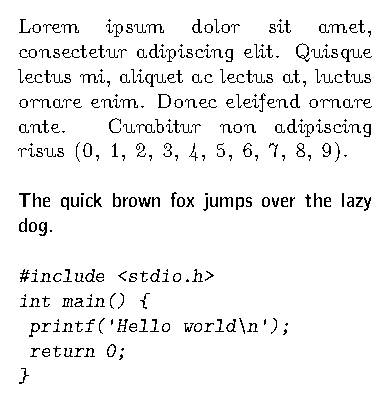
\includegraphics{chapter-4/images/latin-modern-font}\hfill{}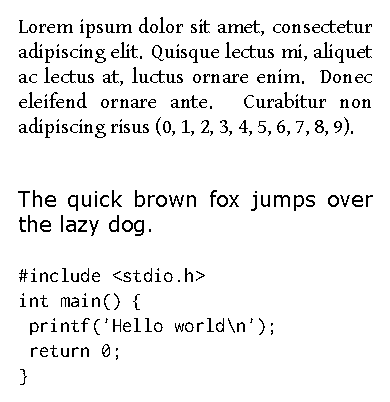
\includegraphics{chapter-4/images/funny-combination-font}

\caption{\label{fig:font-styles}Two different font styles}
\end{figure}
The fonts used in the example are summarized in the Table \ref{tab:font-names}.

\begin{center}
\begin{table}[h]
\centering{}\caption{\label{tab:font-names}Fonts used in the two examples showed before}
\begin{tabular}{lll}
\toprule 
\textbf{Serif} & Latin Modern Roman Unslanted & Gentium\tabularnewline
\textbf{Sans Serif} & Latin Modern Sans Demi Condensed & Verdana\tabularnewline
\textbf{Typewriter} & Latin Modern Mono Slanted & Inconsolata\tabularnewline
\bottomrule
\end{tabular}
\end{table}
\par\end{center}

If, by looking at the \textsf{pdf}, the letters look ugly check the
property of the \textsf{pdf}, in particular the type of fonts used
(how to find this information depends on the \textsf{pdf} viewer that
you are using, if you are using Linux use \textsf{pdffonts} command).
If your \textsf{pdf} has \textsf{Type 3} fonts that is the reason
why your \textsf{pd}f looks ugly. It is better to use \textsf{Type
1} fonts, if you are running \LyX{} on a Linux system by installing
\textsf{cm-super} package you can fix this problem.

\section{Fancy chapter header}

The header of each chapter can be personalized as you like, this requires
you to write a rather big amount of \LaTeX{} code to get a nice result.
However, there is package that provides a set of predefined styles,
\textsf{fncychap} (\url{http://www.ctan.org/pkg/fncychap}). Figure
\ref{fig:fancy-headers} shows just two of the styles offered by the
package.

\begin{center}
\begin{figure}[h]
\begin{centering}
\subfloat[Lenny style]{\centering{}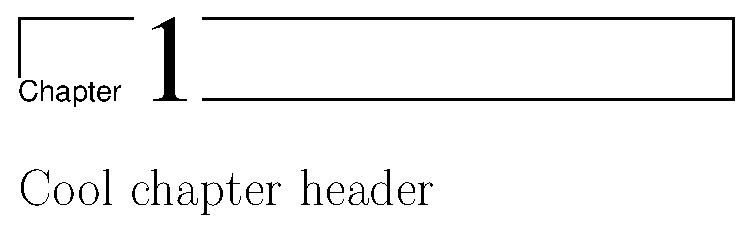
\includegraphics[width=0.6\columnwidth]{chapter-4/images/fancy-page-header-1}}
\par\end{centering}
\begin{centering}
\subfloat[Conny style]{\begin{centering}

\includegraphics[width=0.6\columnwidth]{chapter-4/images/fancy-page-header-2}
\par\end{centering}
}
\par\end{centering}
\caption{\label{fig:fancy-headers}Two possible styles for headers of chapters}
\end{figure}
\par\end{center}

\section{Fancy initial letters}

Another thing that can be fancied are the initial letters. This is
a very simple modification that you can do to add a personal touch
to each chapter. There is a package that permits to customize, with
various options, initial letters called \textsf{lettrine} (\url{http://www.ctan.org/pkg/lettrine}).
There are a lot of options to create your personal style for each
initial, Figure \ref{fig:initial-letters} shows two possible styles
of initials.

\begin{center}
\begin{figure}[h]
\begin{centering}
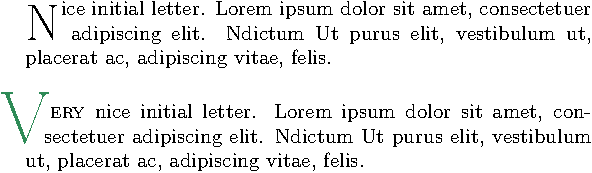
\includegraphics{chapter-4/images/lettrine}
\par\end{centering}
\caption{\label{fig:initial-letters}Two examples of initial letters}
\end{figure}
\par\end{center}

\section{Fancy headers}

Fancy headers are already used in this template, the package used
is \textsf{fancyhdr} (\textsf{\url{http://www.ctan.org/pkg/fancyhdr}}).
There are a lot of options, this template uses almost the standard
style for the header but you can change it. For example, you may move
the page numbering from the bottom header to the top header, or remove
the horizontal line in the header, or \ldots{} . In this template the
fancy header style is set in the \LaTeX{} preamble of the \textsf{thesis.lyx}
document (\textsf{Document} \textsf{\lyxarrow} \textsf{Settings}
\textsf{\lyxarrow} \textsf{\LaTeX{} Preamble}) and just before the
\textsf{Introduction} chapter.

\section{Other document classes}

This template uses the \textsf{book} class, there are some more advanced
classes that have a lot of cool features such as the one offered by
\textsf{koma-script} or \textsf{memoir} (\textsf{\url{http://www.ctan.org/pkg/koma-script}},
\textsf{\url{http://www.ctan.org/pkg/memoir}}).

\LyX{} supports a discrete number of those alternative classes, however
to fully exploit the additional functionalities offered by those classes
you have to write raw \LaTeX{} code. If you want to deeply customize
your thesis maybe it is better if you start considering to write it
directly in \LaTeX{} rather than using \LyX .


\chapter{Fifth chapter\label{chap:fifth-chapter}}




\chapter{Sixth chapter\label{chap:sixth-chapter}}




\chapter{Seventh chapter\label{chap:seventh-chapter}}




\chapter{Eighth chapter\label{chap:eighth-chapter}}




\chapter{Ninth chapter\label{chap:ninth-chapter}}




\chapter*{Conclusions\label{chap:conclusion}}

\addcontentsline{toc}{chapter}{Conclusions}
\markboth{Conclusions}{Conclusions}
\bibliographystyle{plain}
\bibliography{bibliography}
\addcontentsline{toc}{chapter}{Bibliography}

\appendix

\chapter{First appendix\label{app:first-appendix}}




\chapter{Second appendix\label{app:second-appendix}}




\chapter{Third appendix\label{app:third-appendix}}


\cleardoublepage
\end{document}
